% arara: xelatex
% arara: xelatex
% arara: xelatex

% options:
% thesis=B bachelor's thesis
% thesis=M master's thesis
% czech thesis in Czech language
% english thesis in English language
% hidelinks remove colour boxes around hyperlinks

\documentclass[thesis=M,english]{FITthesis}[2019/12/23]

\usepackage[utf8]{inputenc}

\usepackage{graphicx} %graphics files inclusion
\usepackage{wrapfig}
\usepackage{amsmath} %advanced maths
\usepackage{amssymb}
\usepackage{dirtree} %directory tree visualisation
\usepackage{cleveref} % intelligent crossreference
\usepackage{hyperref} % cross-reference
\usepackage{afterpage}
\usepackage{notoccite} % prevent TOC cite 
\usepackage{xcolor}
\usepackage{blindtext}
\usepackage{enumitem}
\usepackage{tabularx} % tables
\usepackage{minted} % code highlight
\usemintedstyle{friendly}

% % list of acronyms
\usepackage[acronym,nonumberlist,toc,numberedsection=autolabel]{glossaries}
\iflanguage{czech}{\renewcommand*{\acronymname}{Seznam pou{\v z}it{\' y}ch zkratek}}{}
\makeglossaries

% Used from http://www.herout.net/blog/2017/03/pomalu-uz-pojdme-psat/
\newglossaryentry{formula}
{
        name=formula,
        description={A mathematical expression}
}
\newcommand{\todo}[1]{\textcolor{red}{\textbf{[#1]}}}
\newcommand{\blind}[1][1]{\textcolor{gray}{\Blindtext[#1][1]}}
\newcommand{\RNum}[1]{\uppercase\expandafter{\romannumeral #1\relax}}

\setlength{\fboxsep}{0.005pt}
\newcommand{\tmpframe}[1]{\fbox{#1}}
%\renewcommand{\tmpframe}[1]{#1} ENABLE WHEN PRINTING


\newcommand{\newpara}
{
  \vskip 0.2in
}

% Q.A env

\newenvironment{questions}{\begin{enumerate}[label=\bfseries\arabic*.]\bfseries}
                      {\end{enumerate}}
\newenvironment{answer}{\par\normalfont}{}

% % % % % % % % % % % % % % % % % % % % % % % % % % % % % % 


\department{Department of Software Engineering}
\title{Coffee Time Mobile Application in Flutter}
\authorGN{Petr} %(křestní) jméno (jména) autora
\authorFN{Nymsa} %příjmení autora
\authorWithDegrees{Bc. Petr Nymsa} %jméno autora včetně akademických titulů
\author{Petr Nymsa} %jméno autora bez akademických titulů
\supervisor{Ing. David Šenkýř}
\acknowledgements{ \todo{todo}Děkuji všem a za vše. Nevíte-li, co sem napsat, příkaz odstraňte.}

\abstractCS{Práce se zabývá využitím multiplatformního frameworku Flutter, umožňující tvorbu aplikací pro mobilní systémy, web i desktop systémy. Hlavním tématem je jeho fungování a~použitelnost při tvorbě aplikací. Flutter je prakticky vyzkoušen na návrhu~a~implementaci aplikace Coffee Time pro operační systém Android a~iOS. Aplikace uživatelům pomáhá vyhledávat kavárny v blízkém okolí s~ možností filtrování dle různých kritérií. 

Práce je zaměřena především na využití frameworku, následný návrh a~implementaci ukázkové aplikace. Kromě použitého frameworku Flutter, aplikace využívá i~serverless přístup pro vývoj serverové části. TODO }

\abstractEN{todo}

\placeForDeclarationOfAuthenticity{Prague}
\declarationOfAuthenticityOption{4} %volba Prohlášení //TODO

\keywordsCS{Flutter framework, reaktivní programování, Android aplikace, vyhledávač kaváren, serverless, Firebase.}

\keywordsEN{Flutter framework, reactive programming, Android application, cafe search, serverless, Firebase.}

\website{http://TODO} %volitelná URL práce, objeví se v tiráži


\begin{document}

% Acronyms and glossary
\newglossaryentry{formula}
{
        name=formula,
        description={A mathematical expression}
}
\newacronym{ctu}{CTU}{Czech Technical University}
\newacronym{cta}{CTA}{Coffee Time API}
\newacronym{gpa}{GPA}{Google Places API}
\newacronym{lofi}{Lo-Fi}{Low Fidelity}
\newacronym{hifi}{Hi-Fi}{High Fidelity}
\newacronym{ui}{UI}{User Interface}

\glsresetall
% % % % % % % % % % % % % % % % % % % % % % % % % % 

\begin{introduction}
The mobile applications usage is growing. The~native development of an application for each, individual platform is well used across many companies. However, many of them, predominantly smaller ones, concludes that developing application for each platform and maintenance is not cheap and comes with much of work. On the~other hand, there are technologies which offer cross-platform development with one code-base. Every cross-platform technology takes its own approach to how the~code is compiled to the~native platform. 

Some of them use the concept of bridging the cross-platform user interface primitives to its counterpart in the native platform. Well-known examples are React~Native~\cite{react-native} or Xamarin~Forms~\cite{xamarin-forms}. The opposite approach is the form of a progressive web application (PWA) where the application is written as a web-based application with support of native features. This approach uses, for example, Ionic framework~\cite{ionic}. 

\begin{figure}[htp]
    \centering
    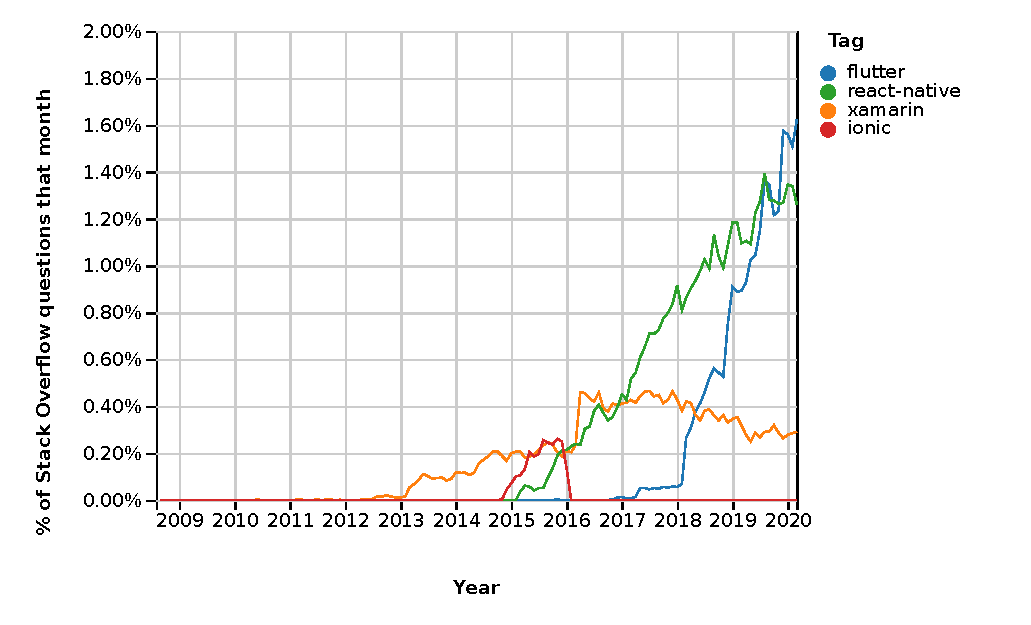
\includegraphics[width=0.88\linewidth]{img/introduction/so-flutter-trend.pdf}
    \caption{Flutter Trend Against Other Popular Frameworks~\cite{so-flutter-trend}.}
    \label{fig:so-flutter-trend}
\end{figure}

During~2017, the~concept of another approach was proposed, where the~application uses low-level platform API to draw over the whole screen with keeping high performance and access to native features. Later on, from this concept open-source framework Flutter, made by Google,  was created~\cite{flutter}. 

Flutter for the last three years until now (first half of 2020) started to gain developers attention, and it was highly promoted by Google. One indication of its growing popularity is \textit{Stack~Overflow Developer Survey~2019}~\cite{so-2019-survey} where it took third place of ``Most Loved'' framework directly after \textit{.NET Core} and \textit{Torch/PyTorch} and highly growing trend among questions created during the last years (\Cref{fig:so-flutter-trend}). However, like with every new technology, the Flutter can become well-known and well used or will be left as a dead-end. 

\section{Motivation}
There are many reasons why the author chose this topic for the thesis. First of all, his bachelor thesis~\cite{nymsap-bp} already focused on mobile application development, although it used different cross-platform technology -- Xamarin. During his ongoing studies, the author discovered and started to use new, by his opinion, promising framework Flutter. So his first goal and motivation was to study Flutter more in-depth and bring comprehensive study material of this framework for others. The second reason was to conclude if Flutter can become a framework which can be used to create production-ready applications or if it is still an experimental framework. Last reason was motivation to create complex, and yet, simple to use mobile application for everyone who seeks to find new cafes to visit.

\section{Structure}
The thesis is divided to four chapters:
\begin{itemize}
\item \Cref{ch:flutter} deals with introduction to Flutter framework, its concept~and internal functionality.
\item \Cref{ch:analysis} introduces proposed Coffee Time application. It describes the~created prototype and its user testing. The~analysis of back-end services is also described. 
\item \Cref{ch:implementation} describes a~process of back-end implementation as well as of Coffee Time application implementation. In the~chapter, details how its implemented, which approaches was taken and how development process was done. 
\item \Cref{ch:testing} describes final application release and its testing. 
\end{itemize}
In conclusion, the results are compared with the goals of this thesis. 
\end{introduction}

\chapter{Flutter Foundations}
\label{ch:flutter}
In the introduction, a new, promising, cross-platform framework was introduced. The Flutter's primary goal is to provide the ability to build high-performance, high-fidelity apps for \textit{iOS}, \textit{Android}, web, and desktop systems (Windows, MacOS) from a single code-base~\cite{flutter-technical-overview}. In this chapter, the~framework philosophy will be described. Used programming language and theory of reactive programming is briefly introduced. The chapter describes the concept of widgets as a base building block for every application. Later on, one of the most critical topics -- \textit{state management} is discussed in the~form of existing approaches and recommendation which to prefer when building applications. At the end of this chapter, the brief look under the framework's hood is discussed.

Flutter includes a modern react-style framework, a 2D rendering engine, predefined widgets and development tools. The primary premise is a motto ``everything is a widget''. A widget is an immutable building block of application which is part of the user interface. Each widget can define structural elements such as a~button, stylistic elements such as colour or it can define the interface's layout, such as padding. Widgets are composed as a tree hierarchy with a~possibility of composing each widget to another. If any event occurs (such as user interaction), the framework can rebuild part of this tree to redraw the screen.  

\begin{figure}[htp]
    \centering
    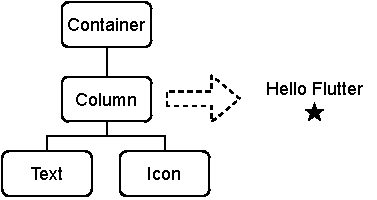
\includegraphics[width=0.5\linewidth]{img/flutter/hello-flutter.pdf}
    \caption{Widget Composition Example.}
    \label{fig:hello-flutter}
\end{figure}

Flutter encourages developers to create and use small, single-purpose widgets and compose them to create complex interfaces and layouts. Take an~example from~\Cref{listing:hello-flutter}, where the root widget, Container, is used to create a rectangular visual element. The Container is something like <div> element in HTML. Under the Container there is Column widget which composes children widgets into the vertical direction. Finally, Text widget displaying text ``Hello Flutter'' and Icon widget showing star icon. The~composition hierarchy along with a~result is shown in~\Cref{fig:hello-flutter}.

\begin{listing}[ht]
\begin{minted}{dart}
Container(
    padding: const EdgeInsets.all(5.0),
    child: Column(
      mainAxisAlignment: MainAxisAlignment.center,
      children: [
        Text('Hello Flutter'),
        Icon(Icons.star),
      ]
    ),
)
\end{minted}
\caption{Widget Composition Code Example.}
\label{listing:hello-flutter}
\end{listing}
% ----- % ----- % ----- % ----- % ----- % ----- % ----- % ----- % ----- % ----- % ----- % ----- % ----- % ----- %
\section{Technical overview}
Flutter uses programming language \textit{Dart}~(specification v2.0~\cite{dart-specs}). It is also made by Google and it is inspired by languages such as JavaScript. Dart using statically typed system with runtime checks, but like many other languages highly use type inference~\cite{dart-type-system}. Dart can be used from writing simple scripts to full-featured applications. Dart has flexible compiler technology where the compiler can decide running code in different ways, depending on the targeted platform~\cite{dart-platforms}. 

\begin{itemize}
    \item \textbf{Dart Native} -- For programs targeting devices (mobile, desktop, server, and more), Dart Native includes both a Dart VM with \gls{jit} compilation and an~\gls{aot} compiler for producing machine code.
    \item \textbf{Dart Web} -- For programs targeting the web, Dart Web includes both a development time compiler (dartdevc) and a production time compiler (dart2js).
\end{itemize}

\begin{figure}[htp]
    \centering
    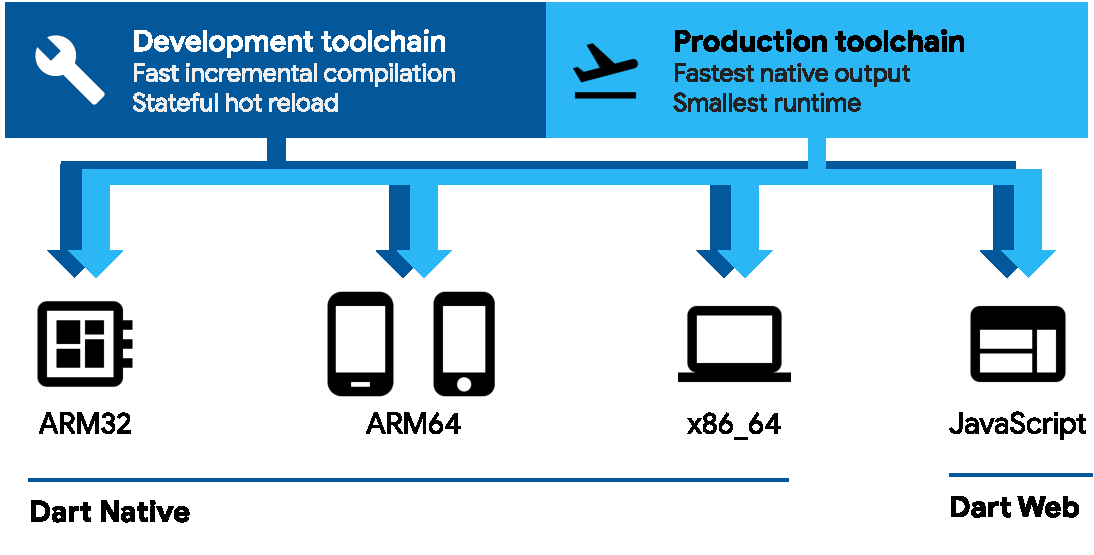
\includegraphics[width=0.8\linewidth]{img/flutter/dart-platforms.pdf}
    \caption{Dart Platforms~\cite{dart-platforms}.}
    \label{fig:dart-platform}
\end{figure}

Flutter performs the use of both ways. If the targeted platform is web, the \textit{Dart~Web} is used. For other platforms \textit{Dart~Native} is chosen. The Dart~Native's \gls{jit} compilation is highly used to support fast development process with ``hot-reload'' functionality. Then the~\gls{aot} compilation is used for the best-optimised production-ready result on the native platform.  

Flutter framework is organised into several layers (see~\Cref{fig:flutter-layer-cake}), where each layer makes usage of the previous one. The upper layers are more frequently used by developers on a daily basis, and lower layers are used only if the developers need to create particular customizations. 

\begin{figure}[htp]
    \centering
    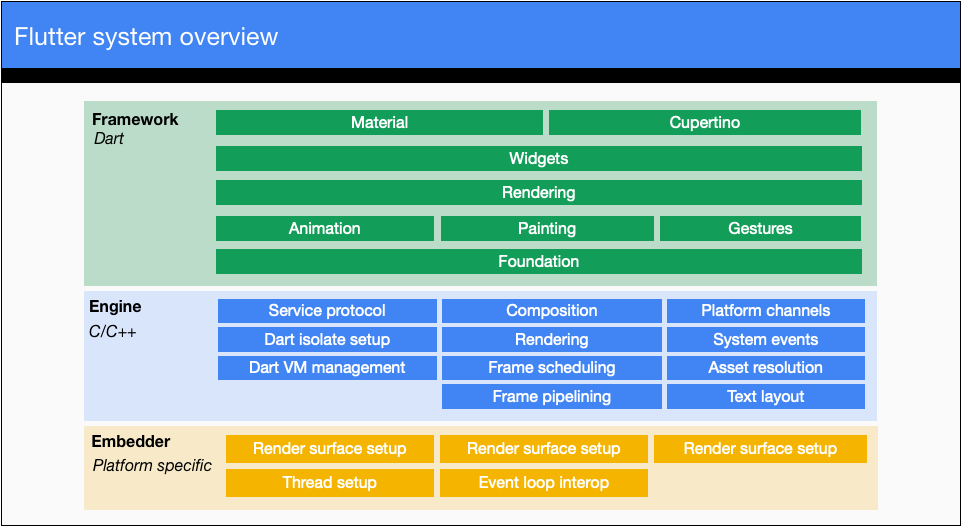
\includegraphics[width=\linewidth]{img/flutter/flutter-layer-cake.png}
    \caption{Flutter System Overview~\cite{flutter-technical-overview}.}
    \label{fig:flutter-layer-cake}
\end{figure}

Unlike the other frameworks, Flutter uses high-performance 2D rendering engine and draws everything onto the~screen directly. That means pixel-perfect control over what and how it is displayed. The most top layers, \textit{Material} and \textit{Cupertino}, are set of widgets which defines Material Design (Android systems) and Apple Design components respectively. To highlight that, Flutter does not use native components, but everything draws by itself. These two layers support developers to bring the standardised look and feel to the targeted platform.
% --- # --- # --- # --- # --- # --- # --- # --- # --- # --- # --- # --- # --- # --- # --- # --- # --- # --- #
\subsection{Reactive Programming}
Flutter makes significant usage from the concept of reactive programming. There is nearly always a~requirement to update data in response to user interaction or any other event such as getting data from the~server. More than that, sometimes it is necessary to update different parts of the user interface in response to these events. 

Flutter creates user interface by composing \textbf{immutable} widgets. The~immutability is the key point here. Whenever user interface needs to ``redraw'' screen, the~part of the~widget tree is replaced by \textbf{new} widget instances (in fact, it is not simple as that, and this topic is more deeply discussed later in this chapter). In many other \gls{ui} frameworks, such as \textit{Xamarin}, is usually taken the approach of coupling \gls{ui} components with view-models through concepts such as data binding~\cite{xamarin-data-binding}. That means that whenever \gls{ui} needs to~change, the~components mutate application's state. Flutter takes an~entirely different approach. It can be said ``here is the current state of the~application, draw something on the screen accordingly''.

\subsubsection{The Notion of Streams}
A Stream can be described as ``a pipe with two ends, only one allowing to insert something into it. When something is inserted into the pipe, it flows inside the pipe and goes out by the other end''~\cite{reactive-didier}. The~Stream can convey any~data type, from simple values to~events, complex object or even another stream. The~data can come to the~Stream, for example, from an external data source such as server connection or from events such as user interactions. In Dart, the Streams support manipulating them, filtering, re-grouping, modify data before they are send and much more. This functionality can be used to build reactive \gls{ui}. Flutter has several widgets supporting streams to rebuild part of the~\gls{ui} whenever new data arrived into the~Stream.

The answer to the question ``What is reactive programming?`` could be ``Reactive programming is programming with asynchronous data streams``~\cite{reactive-didier}\cite{reactive-red-hat}. Within Flutter framework, anything from an interaction event (tap, gesture), changes of a variable, messages, everything that may change is conveyed and triggered by streams.

It means that with reactive programming, according to~\cite{reactive-didier}, the~application:

\begin{quote}
    \begin{itemize}
        \item becomes asynchronous,
        \item is architectured around the notion of Streams and their listeners,
        \item when something happens somewhere (an event, a change of a variable) a~notification is sent to a~Stream,
        \item if ``somebody'' listens to that Stream, it will be notified and will take appropriate action(s), whatever its location in the~application.
    \end{itemize}
    
    From Widgets perspective -- Widget does not longer need to know:
    
    \begin{itemize}
        \item what is going to happen next,
        \item who might use this information (no one, one or several Widgets),
        \item where this information might be used (nowhere, same screen, another one, several ones),
        \item when this information might be used (almost directly, after several seconds, never).
    \end{itemize}
\end{quote}

Later on in this chapter, the pattern Business Logic Component (BLoC) is introduced. This pattern uses Streams to manage application life-cycle and they are used for state management.
% ----- % ----- % ----- % ----- % ----- % ----- % ----- % ----- % ----- % ----- % ----- % ----- % ----- % ----- %
\section{Everything Is a Widget}
In this section, we will discuss in more detail how the~\gls{ui} is built. Every \gls{ui} consists of the layout and individual components. The layout defines the screen's base structure, such as a menu on the top and subsequent actions on the bottom. Then the layout is composed of individual components, such as a menu, buttons or icons. Together they create a final interface.

These building blocks in Flutter are called ``Widgets''. Whatever it is simple text, a button, or complex parts of the~layout, such as a~grid with multiple columns and rows -- \textbf{everything is a widget}.  Widgets describe what their view should look like given their current configuration and state. When a widget's state changes, the widget rebuilds its description, which the framework diffs against the previous description in order to determine the minimal changes needed in the underlying render tree to transition from one state to the next one~\cite{flutter-widget-intro}. As the~composition to the~tree implies, each widget has at most one parent and zero or more children widgets. This tree, called ``widget tree'', is in fact, one of the~three trees involved. The~framework has a sophisticated way of decision about how the~trees should be rebuilt and the~screen updated. This behaviour is in more detail described later in this chapter.

The Flutter framework uses only one language to define both the~user interface and business logic as well.  Widgets are Dart class which inherits from some of the widget's base class (typically \textit{StatelessWidget} or \textit{StatefulWidget}). Each widget has a build method which defines how the widget should be built (and drawn on the screen). 
% --- # --- # --- # --- # --- # --- # --- # --- # --- # --- # --- # --- # --- # --- # --- # --- # --- # --- #
\subsection{Widgets Are Not Only Visible Parts}
Widgets are not only visible parts of the \gls{ui} such as clickable buttons, text or icons. The widgets also define layouts such as columns, rows, grids, the margin between other widgets, padding around them and more. 

\begin{figure}[htp]
    \centering
    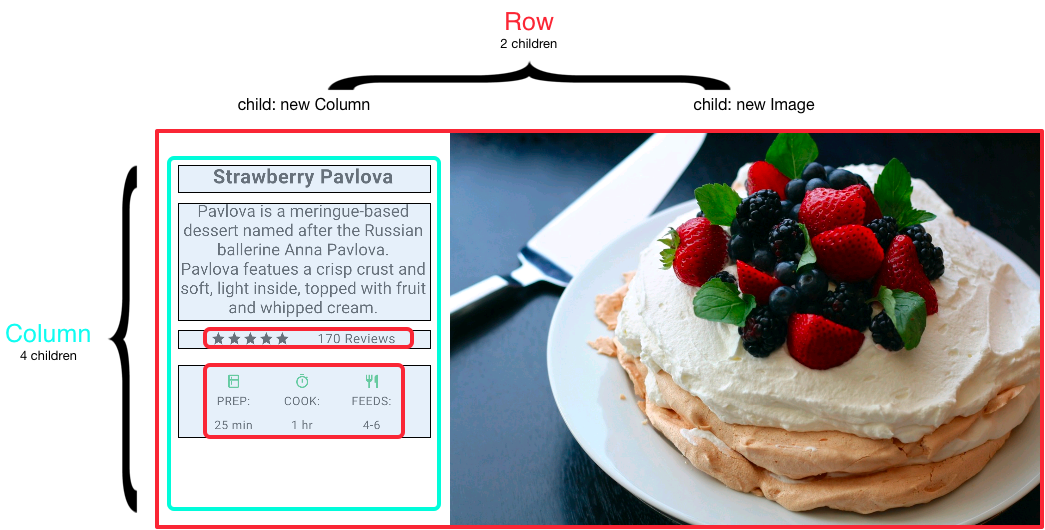
\includegraphics[width=0.9\linewidth]{img/flutter/layout_compose.png}
    \caption{Compose Widgets to Create Layout~\cite{flutter-widget-layout}.}
    \label{fig:flutter-compose-widget}
\end{figure}

An example of widget composition creating a~layout is shown in~\Cref{fig:flutter-compose-widget}. The root widget, a~\textit{Row} widget, contains two nested widgets. On the~left there is a~\textit{Column} which contains more nested widgets and on the~right, \textit{Image} widget which displays a~product image. The~break-down of the left column widget can be seen in~\Cref{fig:flutter-compose-widget-detail}. 

\begin{figure}[htp]
    \centering
    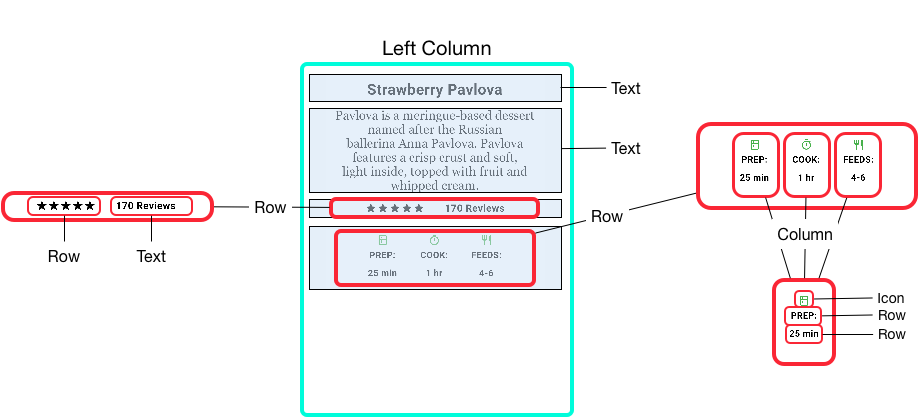
\includegraphics[width=0.9\linewidth]{img/flutter/layout_compose_detail.png}
    \caption{Compose Widgets to Create Layout -- Left Column~\cite{flutter-widget-layout}.}
    \label{fig:flutter-compose-widget-detail}
\end{figure}
% --- # --- # --- # --- # --- # --- # --- # --- # --- # --- # --- # --- # --- # --- # --- # --- # --- # --- #
\subsection{Stateless vs Stateful Widget}
In the introduction it was said that Flutter's approach of displaying current user interface is declarative -- ``here is the current state of the application, draw something on the screen accordingly''.  In Flutter, whenever application' state changes, the user interface is redrawn. There is no imperative changing of the~\gls{ui}, such as \verb|textWidget.text = 'new text'|. The~advantage of the~declarative approach is that there is only one code path for any state of the~\gls{ui}. Developers just describe how the screen should look for a given state, and that is it~\cite{flutter-declarative}. The \gls{ui} can be described as a formula where \gls{ui} is equal to function which takes a state and returns new \gls{ui}~(\Cref{fig:flutter-ui-formula}).

\begin{figure}[htp]
    \centering
    
\includegraphics[width=0.6\linewidth]{img/flutter/ui_f_state.png}
    \caption{User Interface Formula~\cite{flutter-declarative}.}
    \label{fig:flutter-ui-formula}
\end{figure}
% --- & --- & --- & --- & --- & --- & --- & --- & --- & --- & --- & --- & --- & --- & --- & --- & --- & --- &
\subsubsection{Build Context}
An~essential part of the widgets is \textit{BuildContext}. A~context is a~reference to the~location of the~widget within the~part of the~tree~\cite{notion-widget-didier}. Each widget has its own context. As~widgets are composed to the~tree, the contexts are as well. The widget has access to its own context and its parent context. 

The \textit{BuildContext} is provided to each widget through the~build method and is used to find the~widget's ancestors.  This is commonly used to obtain a~defined application theme or get a~reference to a~navigator widget, which is used to do navigation between screens. 
% --- & --- & --- & --- & --- & --- & --- & --- & --- & --- & --- & --- & --- & --- & --- & --- & --- & --- &
\subsubsection{Local vs. Application State}
The state is anything that forms what should be displayed. The state is any data what are needed in order to rebuild \gls{ui} at the~moment~\cite{flutter-local-app-state}. The~state can be separated into two concepts -- local state and application state. 

\begin{itemize}
    \item \textbf{Local state} -- Local state is which can be tied into one widget. It~can be, for example, current tab in the ``tab selector'' widget, current progress of animation or state of checkbox (checked or unchecked).
    \item \textbf{Application state} -- Application State is which can not be local, whenever some information is needed to share across multiple widgets, the~state which should be kept during a~user session. An~example of application state can be a~logged user information, loaded articles from the~server or chat messages.
\end{itemize}
% --- & --- & --- & --- & --- & --- & --- & --- & --- & --- & --- & --- & --- & --- & --- & --- & --- & --- &
\subsubsection{Stateless Widget}
A~Stateless Widget is a widget which does not manage its own state. Once it gets its parameters, and it was built through the build method, it cannot be changed. Remember, that whenever Flutter decides to redraw the~screen, part of the~tree is rebuilt, but with new instances of the~widgets. Typical examples of the Stateless Widgets can be \textit{Container}, \textit{Text} or \textit{Icon}. These widgets accept many parameters which can alter their look (and behaviour), but they cannot be changed later on by~themselves. 
% --- & --- & --- & --- & --- & --- & --- & --- & --- & --- & --- & --- & --- & --- & --- & --- & --- & --- &
\subsubsection{Stateful Widget}
Whenever widget needs to manage its state and wants to mutate it for example, in case of an event, the widget should be stateful.  The widget as a~Stateless accepts parameters which can be used to configure this widget but also has an associated object, called state. This state object is an active part of the widget and is used to change widget and force framework rebuilt\gls{ui}. An~example of a \textit{Stateful Widget} can be a checkbox with ``checked'' state. 

Stateful Widget does not have only \verb|build()| method but has associated State object which defines several methods to support widget's lifecycle. These methods are \verb|initState()| for any state initialisation and \verb|dispose()| to clear any allocated resources. 

The state object is associated with widget's \textit{BuildContext}. This association is permanent, and state object will never change it~\cite{notion-widget-didier}. Even if the~Widget's \textit{BuildContext} can be moved around the~tree structure, the~state will remain associated with that context. This implies that, the~Stateful Widget can be replaced during the~tree rebuild with new a~instance, but the~state object is persisted. 
% --- & --- & --- & --- & --- & --- & --- & --- & --- & --- & --- & --- & --- & --- & --- & --- & --- & --- &
\subsubsection{Force Rebuild with setState()}
As was mentioned, Stateful Widget can tell the framework to rebuild, and the widget can be redrawn based on the~changed state. The~Stateful Widget has method \verb|setState(callback)| which is used to do such rebuild. Inside \verb|callback| a developer should change the~widget's state to the~new value and framework will rebuild the widget based on that~new state. 
% --- & --- & --- & --- & --- & --- & --- & --- & --- & --- & --- & --- & --- & --- & --- & --- & --- & --- &
\subsubsection{Case Study: Counter Application}
Suppose application where are two buttons. One button increments a value (\verb|counter|) and other decrements. The counter value is displayed within two Text widgets located on different places within the application. Whenever any of the buttons are clicked, and the value is changed, all Text widgets should reflect this change.

\begin{figure}[htp]
    \centering
    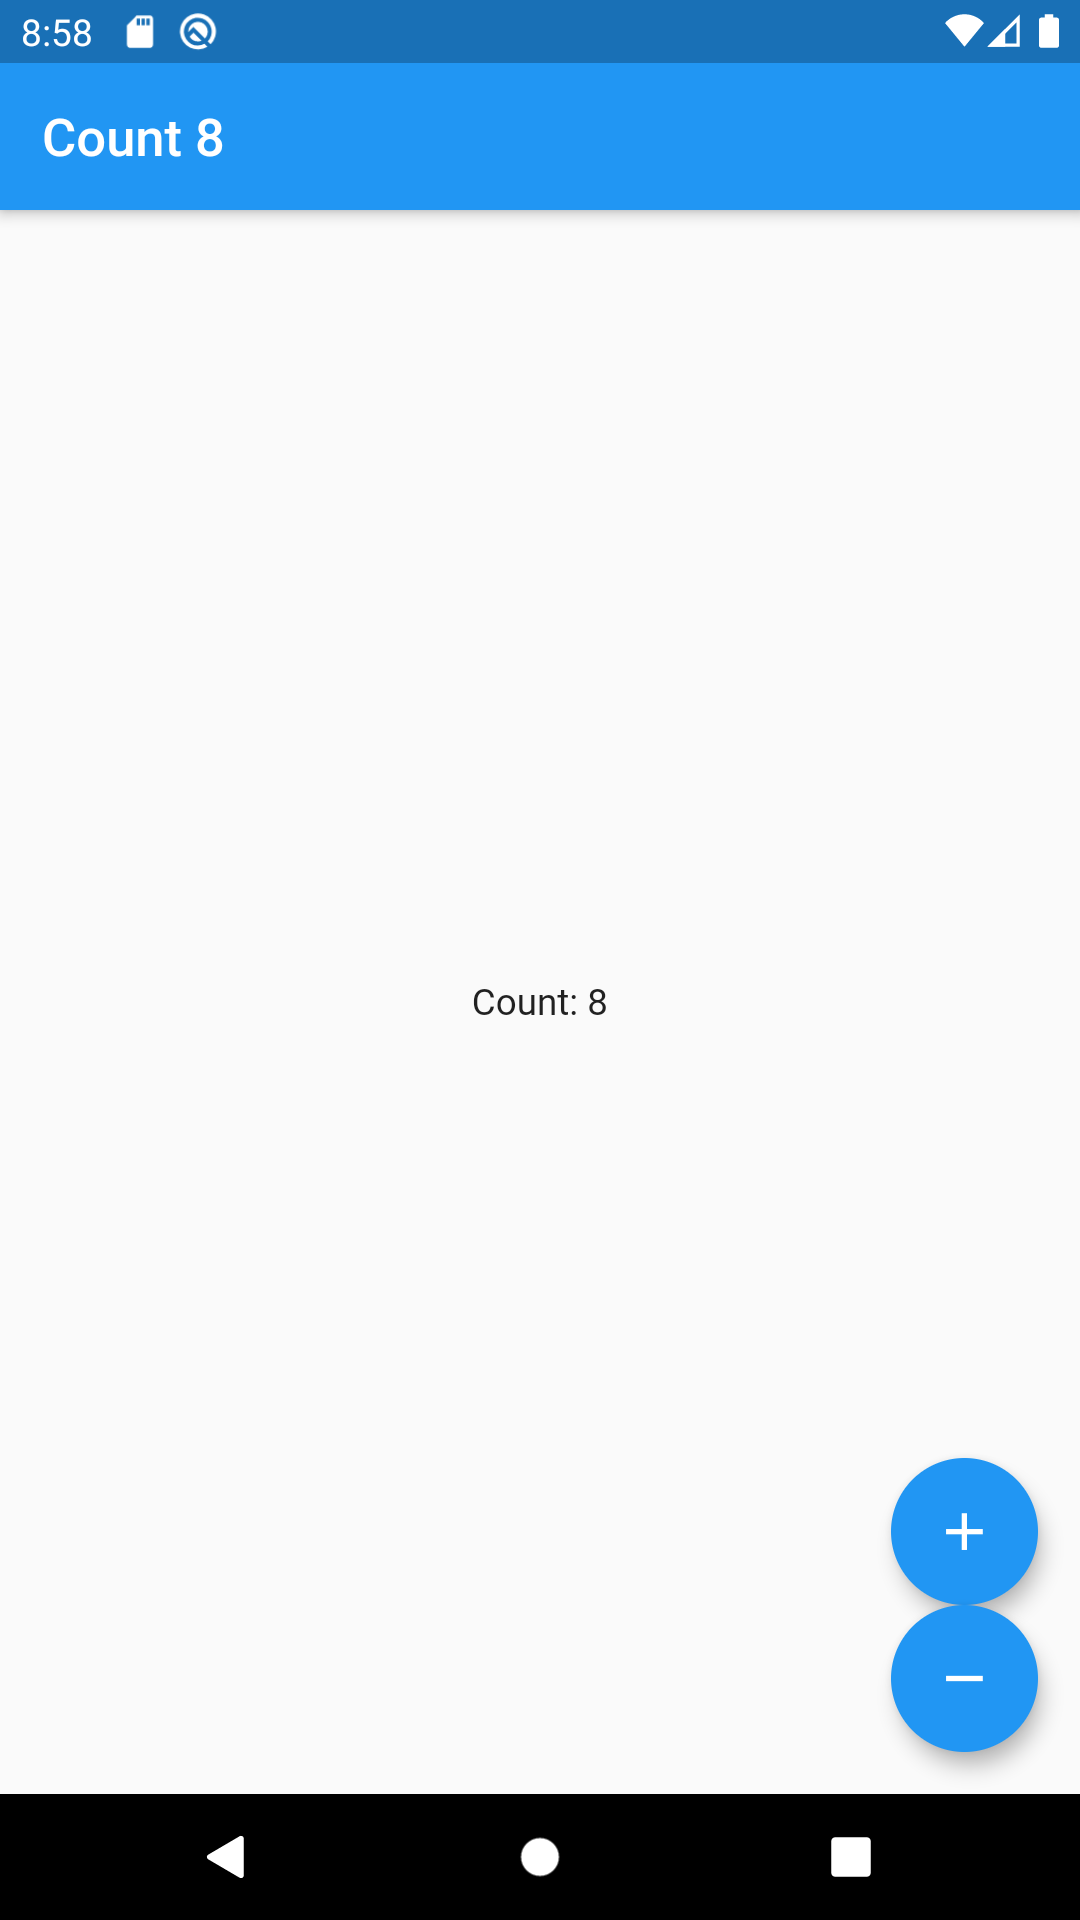
\includegraphics[width=0.33\linewidth]{img/flutter/counter_app_base.png}
    \caption{Counter Application.}
    \label{fig:counter-app}
\end{figure}

\begin{figure}[htp]
    \centering
    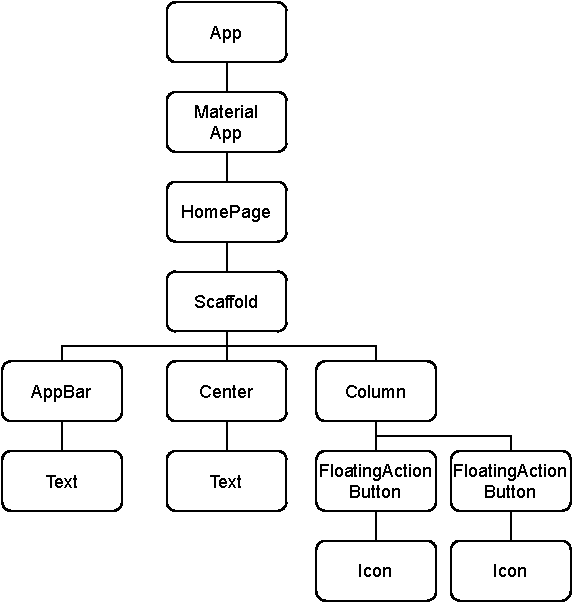
\includegraphics[width=0.75\linewidth]{img/flutter/counter-base.pdf}
    \caption{Counter Application's Widget Tree.}
    \label{fig:counter-app-widget-tree}
\end{figure}

Application's layout is shown in~\Cref{fig:counter-app} and the~corresponding widget tree in~\Cref{fig:counter-app-widget-tree} (shortened for brevity). In the \textit{AppBar} and in the centre of the screen, there is \textit{Text} widget which displays current value. On the bottom of the screen there are \textit{FloatingActionButtons} widgets, which increment (decrement) counter value. The value needs to be accessible to the Text and to the button as well. Hence, the state is declared within the whole application's widget \textit{HomePage}.  

\begin{listing}[ht]
\begin{minted}{dart}
class HomePage extends StatefulWidget {
  @override
  _HomePageState createState() => _HomePageState();
}
\end{minted}
\caption{HomePage Widget Definition.}
\label{listing:counter-homepage-widget}
\end{listing}

\Cref{listing:counter-homepage-widget} shows the definition of the \textit{HomePage} widget. The widget inherits from \verb|StatefulWidget| and declares \textit{HomePageState} which is an associated state object.

\begin{listing}[ht]
\begin{minted}{dart}
class _HomePageState extends State<HomePage> {
  int _counter = 0;
  void _incrementCounter() => setState(() => _counter++);
  void _decrementCounter() => setState(() => _counter--);

  @override
  Widget build(BuildContext context) {
    return Scaffold(
      appBar: AppBar(title: CounterTextContainer(_counter)),
      body: Center(child: CounterTextContainer(_counter)),
      floatingActionButton: Column(
        children: <Widget>[
          FloatingActionButton(
            onPressed: _incrementCounter,
            child: Icon(Icons.add),
          ),
          FloatingActionButton(
            onPressed: _decrementCounter,
            child: Icon(Icons.remove),
          )]));
   }
}
\end{minted}
\caption{HomePageState -- setState() Example.}
\label{listing:counter-base-state-homepage}
\end{listing}

\begin{listing}[ht]
\begin{minted}{dart}
class CounterTextContainer extends StatelessWidget {
  final int count;
  CounterTextContainer(this.count);
  
  @override
  Widget build(BuildContext context) {
    return Row(
        children: [
          const Icon(Icons.computer),
          const SizedBox(width: 5),
          Text('Count: $count')
        ],
    );
  }
}
\end{minted}
\caption{CounterTextContainer -- Accepting State As Parameter}
\label{listing:counter-base-text-container}
\end{listing}

\begin{figure}[htp]
    \centering
    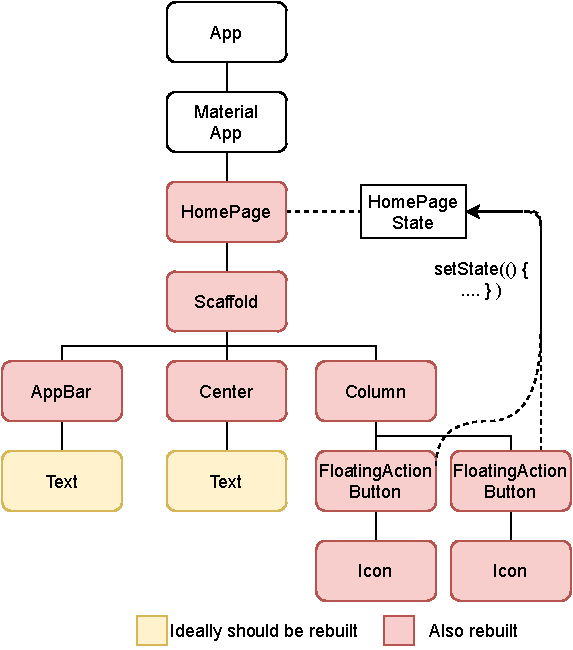
\includegraphics[width=0.75\linewidth]{img/flutter/counter-base-setState.pdf}
    \caption{Expected Rebuilt vs Actual Rebuilt.}
    \label{fig:counter-app-base-build}
\end{figure}

\Cref{listing:counter-base-state-homepage} shows definition of \textit{HomePageState} where state is represented as \verb|int _counter = 0| variable. There are also two private methods for incrementing and decrementing counter value. In each of the methods, the \verb|setState()| is called with the appropriate state change.  These two methods are bound to \verb|onPressed()| callback within \textit{FloatingActionButton}. The~state (\verb|_counter| variable) is passed down to~\verb|CounterTextContainer|~\Cref{listing:counter-base-text-container} where the value is used to display within \textit{Text} widget. 

The expectation is, that if the user pressed any of the buttons, the value is increment or decremented respectively and part of \gls{ui} which depends on \verb|_counter| value will be rebuilt. This part should be two Text widgets. In fact, the state is defined within the~\textit{HomePage} widget, and so, the~whole \textit{HomePage} and its children are rebuilt~(\Cref{fig:counter-app-base-build}). In~this small example, it is not really a~problem and performance should not be affected. However, if the~tree is deeply nested with heavy performance widgets (for example animations), it could lead to reduced performance and application can lags. 

How to define the application-wide state and prevent the necessary rebuilding part of the widget tree is a subject of ``state management'' section.
% ----- % ----- % ----- % ----- % ----- % ----- % ----- % ----- % ----- % ----- % ----- % ----- % ----- % ----- %
\section{State Management Approaches}
Using \verb|setState()| method is the~perfect solution (and recommended) for local state. However, as~soon as the state needs to be shared across multiple widgets, the managing this state becomes cumbersome. If the~state should be shared, there is only one viable solution -- \textbf{lifting state up}~\cite{flutter-simple-state-management}. The~state should reside in the widget, which is the parent for all widgets that needs access to the~state. Such a~solution can be used (and works) but creates a~few problems. 

The~very first problem is if some of the~interested widgets are kept in deep layers of the~tree and others are not, the~necessary amount of widgets is rebuilt whenever the state changes. The~second issue is that the~code of the widgets becomes very quickly hard to~manage due to its tight dependencies with upper widgets. The only doable solution to provide access to the~state is through references or function callbacks. These callbacks have to be passed to every widget down to the tree. This solution adds the~necessary complexity to maintenance and readability. Last but not least, the~application state usually has some business logic which should have been tested. However, if the~state (and its logic) is put directly into the widget, this logic is hard to test. 

The ``State Management'' is a~term for patterns and design solutions which helps to prevent those issues -- reducing necessary rebuilds, keeping code maintainable and testable. 
% --- # --- # --- # --- # --- # --- # --- # --- # --- # --- # --- # --- # --- # --- # --- # --- # --- # --- #
\subsection{Case Study Note}
In our case study, there are two places where the state (counter value) is needed -- first place is in the~AppBar's text and the centre of the screen. Secondly, the buttons for incrementing and decrementing need access to the~state in order to modify it. The first version of counter application used solution with \verb|setState()| and made the \textit{HomePage} (a root widget of the whole application) as \textit{StatefulWidget}. The~state was then accessible from every HomePage's children. Although this code is straightforward, there is already an~issue with the testability of the~business logic as it is tightly coupled to widget's class.  

Following lines in this section introduce some used patterns and solutions for state management.  Every solution will use the same case study but with appropriate implementation. Each solution's full code is available as an~appendix. The design and functionality remain the same as introduced before.
% --- # --- # --- # --- # --- # --- # --- # --- # --- # --- # --- # --- # --- # --- # --- # --- # --- # --- #
\subsection{Inherited Widget}
One solution offered by \textit{Flutter} framework is the concept of \textit{InheritedWidget}~\cite{flutter-inherited-widget}~\cite{notion-widget-didier}. This concept is used across the framework -- for example, obtaining current \textit{Theme} or screen device information through \textit{MediaQuery} object. Both can be accessed through convention ``of'' method -- \verb|Theme.of(context)| returns \textit{Theme} object. Internally these objects makes usage of InheritedWidget. InheritedWidget has two features:

\begin{itemize}
    \item It can be accessed from any widget directly.
    \item Whenever the widget changes, the accessing widget is automatically rebuilt.
\end{itemize}

The second implies that, for example, whenever widget access the~\textit{MediaQuery} and it is changed (the device is rotated, resolution changed,\ldots ), the widget is rebuilt to handle these changes. 

\begin{listing}[ht]
\begin{minted}{dart}
class _CounterInherited extends InheritedWidget {
  _CounterInherited({Widget child, this.data}) 
        : super(child: child);

  final CounterModel data;

  @override
  bool updateShouldNotify(_CounterInherited oldWidget) => true;
}
\end{minted}
\caption{\_CounterInherited.}
\label{listing:counter-inherited-counter-inherited}
\end{listing}

\begin{listing}[ht]
\begin{minted}{dart}
class CounterModelProvider extends StatefulWidget {
  CounterModelProvider({this.child});
  
  final Widget child;
  
  @override
  CounterModel createState() => CounterModel();

  static CounterModel of(BuildContext context, 
                         {bool listen = true}) {
    return (listen
        ? context.
            dependOnInheritedWidgetOfExactType<_CounterInherited>()
        : context.
            findAncestorWidgetOfExactType<_CounterInherited>()
        )
        .data;
  }
}
\end{minted}
\caption{CounterModelProvider.}
\label{listing:counter-inherited-model-provider}
\end{listing}

\begin{listing}[ht]
\begin{minted}{dart}
class CounterModel extends State<CounterModelProvider> {
  int _count = 0;
  int get count => _count;

  void increment() => setState(() => _count++);
  void decrement() => setState(() => _count--);

  @override
  Widget build(BuildContext context) {
    return _CounterInherited(data: this, child: widget.child);
  }
}
\end{minted}
\caption{CounterModel.}
\label{listing:counter-inherited-counter-model}
\end{listing}

\Cref{listing:counter-inherited-counter-inherited} is implementation of \textit{InheritedWidget}. It accepts child widget and \verb|CounterModel| which is state (and business logic) holding class (\Cref{listing:counter-inherited-counter-model}). The \verb|CounterModelProvider|~(\Cref{listing:counter-inherited-model-provider}) is a~widget which provides \verb|of(context, listen)| method and should be called when widget needs access to the model. The optional parameter \verb|listen| controls if a widget is automatically assigned to listening for changes or not. The \verb|of| method make usage of \verb|BuildContext| and traverses from given widget up to the~root until it finds the~widget searched for or fails. 

\begin{listing}[ht]
\begin{minted}{dart}
// MyApp - wraping HomePage with CounterModelProvider
home: CounterModelProvider(child: HomePage()),
// HomePage's build method
final model = CounterModelProvider.of(context, listen: false);
return Scaffold(
    appBar: AppBar(title: CounterTextContainer()),
    body: Center(child: CounterTextContainer()),
    floatingActionButton: Column(
      children: [
        FloatingActionButton(
          onPressed: model.increment,
          child: Icon(Icons.add),
        ),
        FloatingActionButton(
          onPressed: model.decrement,
          child: Icon(Icons.remove),
        )
      ],
));
\end{minted}
\caption{HomePage Implementation.}
\label{listing:counter-inherited-homepage}
\end{listing}

\begin{listing}[ht]
\begin{minted}{dart}
// CounterTextContainer's build method
return Row(
    children: [
      const Icon(Icons.computer),
      const SizedBox(width: 5),
      CounterText()
    ]);
//CounterText's build method
final model = CounterModelProvider.of(context);
return Text('Count: ${model.count}');
\end{minted}
\caption{CounterTextContainer and CounterText Widgets.}
\label{listing:counter-inherited-text-container}
\end{listing}

\begin{figure}[htp]
    \centering
    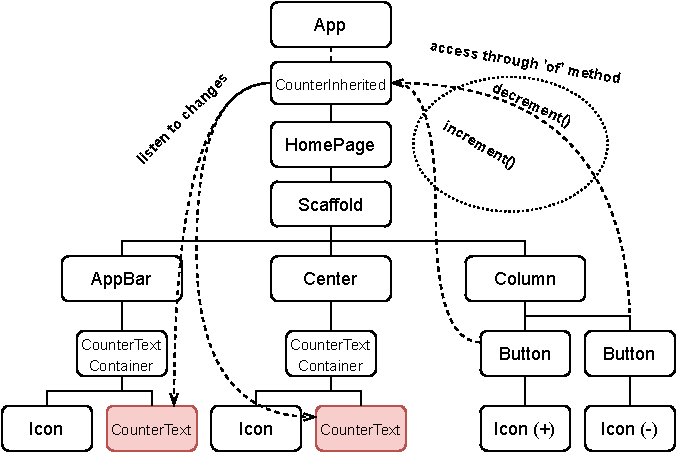
\includegraphics[width=0.75\linewidth]{img/flutter/counter-inherited-widget.pdf}
    \caption{InheritedWidget Approach and Its Widget Tree.}
    \label{fig:counter-app-inherited-widget}
\end{figure}

The HomePage~(\Cref{listing:counter-inherited-homepage}) is wrapped by~\verb|CounterModelProvider| to provide access to any its children. Within the HomePage's \verb|build()| method, \verb|CounterModel| is obtained without listening. It is used for button's callbacks to invoke \verb|increment()| (\verb|decrement()| respectively) method. Inside \verb|CounterTextContainer| (\Cref{listing:counter-inherited-text-container}) is used Text widget and \verb|CounterText| where the~\verb|CounterModel| is accessed to get current value. Note that every widget is Stateless. The~most important thing is that only the~\textit{CounterText is~rebuilt} when the~state changes~(see~\Cref{fig:counter-app-inherited-widget}) in comparison with \verb|setState| approach where the~whole application was rebuilt.

Although InheritedWidget solves many issues, the amount of code needed to achieve these results can be more unreadable and hard to maintain than approach with plain \verb|setState| method. However, Flutter's community created package which abstracts InheritedWidget and simplify this process. 
% --- # --- # --- # --- # --- # --- # --- # --- # --- # --- # --- # --- # --- # --- # --- # --- # --- # --- #
\subsection{Provider Package}

\begin{listing}[ht]
\begin{minted}{dart}
class CounterModel with ChangeNotifier {
  int _count = 0;
  int get count => _count;

  void increment() {
    _count++;
    notifyListeners();
  }

  void decrement() {
    _count--;
    notifyListeners();
  }
}
\end{minted}
\caption{Provider's CounterModel.}
\label{listing:counter-provider-model}
\end{listing}

\begin{listing}[ht]
\begin{minted}{dart}
// in MyApp: provides CounterModel to descendants
home: ChangeNotifierProvider(
    create: (_) => CounterModel(),
    child: HomePage(),
),
// HomePage's build method
final model = Provider.of<CounterModel>(context, listen: false);
// ... rest of the HomePage's build method
// ... which is same as within InheritedWidget approach
\end{minted}
\caption{Provider's HomePage.}
\label{listing:counter-provider-home-page}
\end{listing}

\begin{listing}[ht]
\begin{minted}{dart}
//CounterTextContainer build method
return Consumer<CounterModel>(
  builder: (context, model, child) {
    return Row(
        children: [
          child,
          const SizedBox(width: 5),
          Text('Count: ${model.count}') // CounterText
        ]);
  },
  // child widget is not rebuilt when model changes
  child: Container(
    padding: const EdgeInsets.all(8.0),
    child: Icon(Icons.computer),
  ),
);
\end{minted}
\caption{CounterTextContainer with Consumer.}
\label{listing:counter-provider-consumer}
\end{listing}

\begin{figure}[ht]
    \centering
    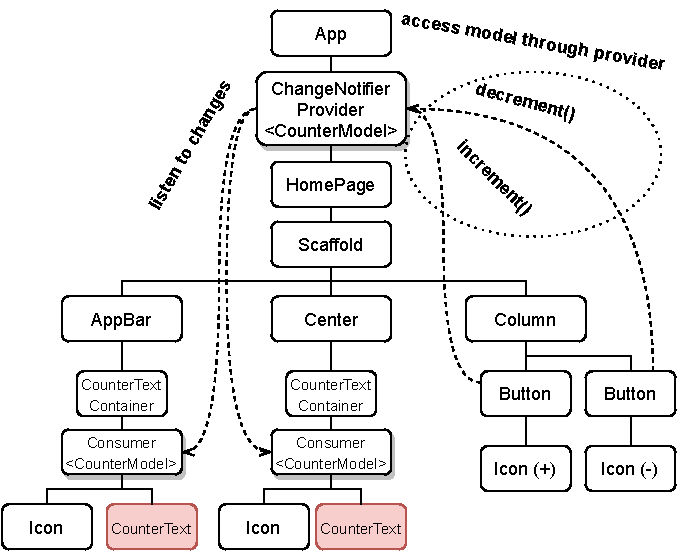
\includegraphics[width=0.75\linewidth]{img/flutter/counter-provider.pdf}
    \caption{Provider Approach and Its Widget Tree.}
    \label{fig:counter-app-provider}
\end{figure}

Provider is a community package created by \textit{Remi~Rousselet}~\cite{package-provider} as a~simplification over inherited widgets with abstraction and more flexibility. One of the features is the concept of \verb|ChangeNotifier| and its \verb|ChangeNotifierProvider|. The concept behind is similar to the approach with the \verb|InheritedWidget|. The state is represented by the model class \verb|CounterModel|, which uses mixin \verb|ChangeNotifier|~(\Cref{listing:counter-provider-model}). This model contains only business logic and associated data. There are no widgets involved. If any of value is changed, the \verb|notifyListeners()| method should be called to notify its listeners to rebuilt.

The~\verb|ChangeNotifierProvider| wraps HomePage widget, where \verb|CounterModel| is created. Within HomePage's build method, the \verb|CounterModel| is accessed through \verb|Provider.of<CounterModel>(context, listen: false);| \\(note the~similarity with InheritedWidget) without listening to changes~(\Cref{listing:counter-provider-home-page}). The \verb|Consumer| widget used within \verb|CounterTextContainer|~(\Cref{listing:counter-provider-consumer}) allows to automatically listening to changes and re-run its \verb|builder| callback. If needed, the \verb|child| argument can be used to construct widget which can be part of the rebuilding widget without rebuilding itself. 

The result is the same as with \verb|InheritedWidget|~(\Cref{fig:counter-app-provider}), but with more readable code. The~\textit{Provider} package became very popular and encouraged by the Flutter team as a~solution for state management~\cite{flutter-simple-state-management}. Package offers more than the~\verb|ChangeNotifier| -- it can be used for dependency injection and it is used by many other packages such as~\textit{flutter\_bloc}~\cite{package-bloc}.
% --- # --- # --- # --- # --- # --- # --- # --- # --- # --- # --- # --- # --- # --- # --- # --- # --- # --- #
\subsection{Business Logic Component}
\gls{bloc} is a~pattern originally introduced by~\textit{Paolo Soares} and presented during \textit{DartConf~2018} conference~\cite{bloc-pattern-youtube}. The pattern was popularized by~\textit{Didier Boelens}~\cite{reactive-didier} and it was inspiration to \textit{Felix Angelov} for creation of~\textit{flutter\_bloc} package~\cite{package-bloc} -- a~popular BLoC based state management solution.

\begin{figure}[ht]
    \centering
    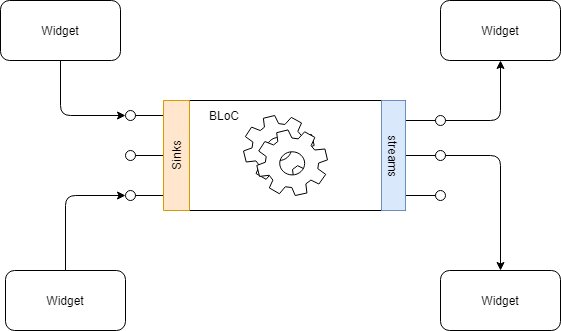
\includegraphics[width=0.6\linewidth]{img/flutter/bloc_pattern.png}
    \caption{A BLoC Pattern~\cite{notion-widget-didier}.}
    \label{fig:bloc-pattern}
\end{figure}

The \gls{bloc} builds on the streams. The \gls{bloc} stands for class, holding business logic where on one side accepts stream of events (event sink) and on the other side provides stream of states~(\Cref{fig:bloc-pattern}). Through event sinks, \gls{bloc} accepts events which are processed and based on them a new state is put to the state stream. In terms of Flutter -- widgets send events and listens for new state coming from state stream. The business logic itself is hidden from them and widgets (the~\gls{ui}) are concerned only about sending event and rebuilding themselves based on coming state.

The~\gls{bloc} solves the responsibility separation where the logic is centralised within the~\gls{bloc} class. This leads to better and easier testability. And~third, thanks to the~independence of \gls{ui} with business logic, changing and organizing layouts can be done without changes within the application's logic. The~\gls{ui} is only concerned about building widgets based on the current state and eventually sending events if needed. This also imply that events can be sent from any place within the application without any complexity.

\begin{figure}[ht]
    \centering
    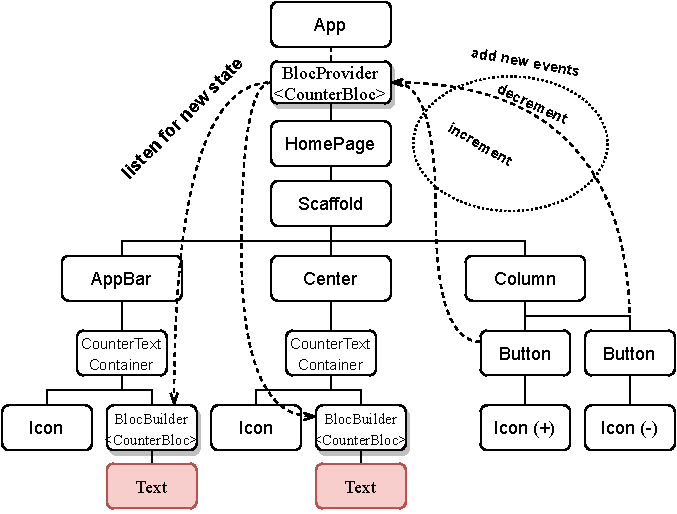
\includegraphics[width=0.75\linewidth]{img/flutter/counter-bloc.pdf}
    \caption{BLoC Approach and Its Widget Tree.}
    \label{fig:counter-app-bloc}
\end{figure}

The \gls{bloc} also force centralized place where the particular state can be changed. With other solutions such as \textit{setState} and eventual callback passing, these changes can be spread across many places and it can be hard to maintain and test them. On the~other hand, the~usage of streams adds code complexity and robustness -- a~code boilerplate and the~application has to be designed with asynchronous execution in mind as the~\gls{bloc} relies on the~streams. The mentioned package \textit{flutter\_bloc} is \gls{bloc} pattern with abstraction over the stream's complexity without downgrading their usefulness and advantages. 

\subsubsection{flutter\_bloc Package}
\begin{listing}[ht]
\begin{minted}{dart}
// CounterBloc's events
enum CounterEvent { increment, decrement }

class CounterBloc extends Bloc<CounterEvent, int> {
  @override int get initialState => 0;

  @override
  Stream<int> mapEventToState(
    CounterEvent event,
  ) async* {
    if (event == CounterEvent.increment)
      yield state + 1;
    else if (event == CounterEvent.decrement) yield state - 1;
  }
}
\end{minted}
\caption{CounterBloc's Implementation.}
\label{listing:counter-bloc-bloc}
\end{listing}

\begin{listing}[ht]
\begin{minted}{dart}
// App' build method -- providing CounterBloc
home: BlocProvider(
        create: (_) => CounterBloc(),
        child: HomePage()),
        
// inside onPressed() callback - add event to bloc
context.bloc<CounterBloc>().add(CounterEvent.increment),
\end{minted}
\caption{BLoC Approach -- Providing CounterBloc and Accessing Bloc.}
\label{listing:counter-bloc-homepage}
\end{listing}

As before, the case study ``counter application'' was also written with the~\gls{bloc} approach. Widget tree and its rebuild~(\Cref{fig:counter-app-bloc}) is practically identical as with Provider. The difference lies in the how the code is organised, how the state is managed and the whole philosophy of the application's code. With \verb|InheritedWidget| the~state was mutated and its listeners were notified. With \gls{bloc} approach, whenever arrives new state, new state is returned and its listeners are rebuilt. 

\begin{listing}[ht]
\begin{minted}{dart}
Row(
children: <Widget>[
  const Icon(Icons.computer),
  const SizedBox(width: 5),
  BlocBuilder<CounterBloc, int>(
    builder: (context, state) => Text('Count: $state'),
  )]);
\end{minted}
\caption{BLoC Approach -- CounterTextContainer's Implementation.}
\label{listing:counter-bloc-counter-text}
\end{listing}

The~\verb|flutter_bloc| has base \verb|Bloc<E,S>| class where \verb|E| is an ``event type'' and \verb|S| is a ``state type''. Each \gls{bloc} class has to inherit this base class and overrides ``mapEventToState'' method in order to respond to any event and \textit{yield} new state. How the~package works and how it can be used is more discussed in~\Cref{ch:implementation}. \Cref{listing:counter-bloc-bloc} shows \verb|CounterBloc| implementation. Events are represented as enum \verb|CounterEvent| with \textit{increment} and \textit{decrement} respectively. The state is simple \textit{integer} type. The \verb|flutter_bloc| package uses under the~hood \textit{Provider} so it is very similar how the~\gls{bloc} is provided to the widget tree. The bloc is accessed with \verb|context.bloc| in order to add new events. An example is shown at~\Cref{listing:counter-bloc-homepage}.  \verb|CounterTextContainer| widget (\Cref{listing:counter-bloc-counter-text}) uses \verb|BlocBuilder| widget which rebuilds whenever new state arrives. 
% --- # --- # --- # --- # --- # --- # --- # --- # --- # --- # --- # --- # --- # --- # --- # --- # --- # --- #
\subsection{Conclusion}
In this section, four approaches for state management was introduced. From simple \verb|setState| approach to stream based \gls{bloc}. As the \gls{bloc} encapsulates business logic into its own class and makes use of stream notion, this approach was chosen as the state management approach for implementation of our application due to convenient and straightforward way to usage, along with easy testability.
% ----- % ----- % ----- % ----- % ----- % ----- % ----- % ----- % ----- % ----- % ----- % ----- % ----- % ----- %
% \section{Native Features}
% \todo{How flutter can use native functions, e.g camera. Flutter plugins.}
% ----- % ----- % ----- % ----- % ----- % ----- % ----- % ----- % ----- % ----- % ----- % ----- % ----- % ----- %
\section{Flutter Internals}
In the last section of this chapter, some of the~internal Flutter's work is discussed. First of all, it is described more in-depth on how the framework is able to build widgets and draw them on the screen. Then the notion of Keys is introduced (an unique identification of widgets within widget tree). After that some optimisations such as const constructors which can give better performance are discussed. 

At the beginning of this chapter, \Cref{fig:flutter-layer-cake} shows how the Flutter is made. The middle layer - the engine is responsible for rendering and orchestrating Flutter framework. 
% --- # --- # --- # --- # --- # --- # --- # --- # --- # --- # --- # --- # --- # --- # --- # --- # --- # --- #
\subsection{RenderObject and RenderTree}
As was said earlier, Flutter uses pixel-perfect rendering -- each Widget is in the end translated into several pixels drawn on the screen. In order to do that, engine has a notion of the Render Tree.

The RenderTree is composed by objects called RenderObjects. These RenderObjects are used to define~\cite{didier-internals}:
\begin{itemize}
    \item define some area of the screen in terms of dimensions, position, geometry but also in terms of ``rendered content'',
    \item identify zones of the screen potentially impacted by the gestures,
\end{itemize}
The root object of the tree is called RenderView.
% --- # --- # --- # --- # --- # --- # --- # --- # --- # --- # --- # --- # --- # --- # --- # --- # --- # --- #
\subsection{Everything is a Widget Revisited}
From a developer perspective, everything is a widget what is related to the~\gls{ui} in terms of layout and interaction~\cite{didier-internals}. The~Widget is an immutable class, where instances (or more precise its derivates) form the widget tree by composition. The~Widget itself, however, does not know how it can be rendered to the~screen. 

\begin{figure}[ht]
    \centering
    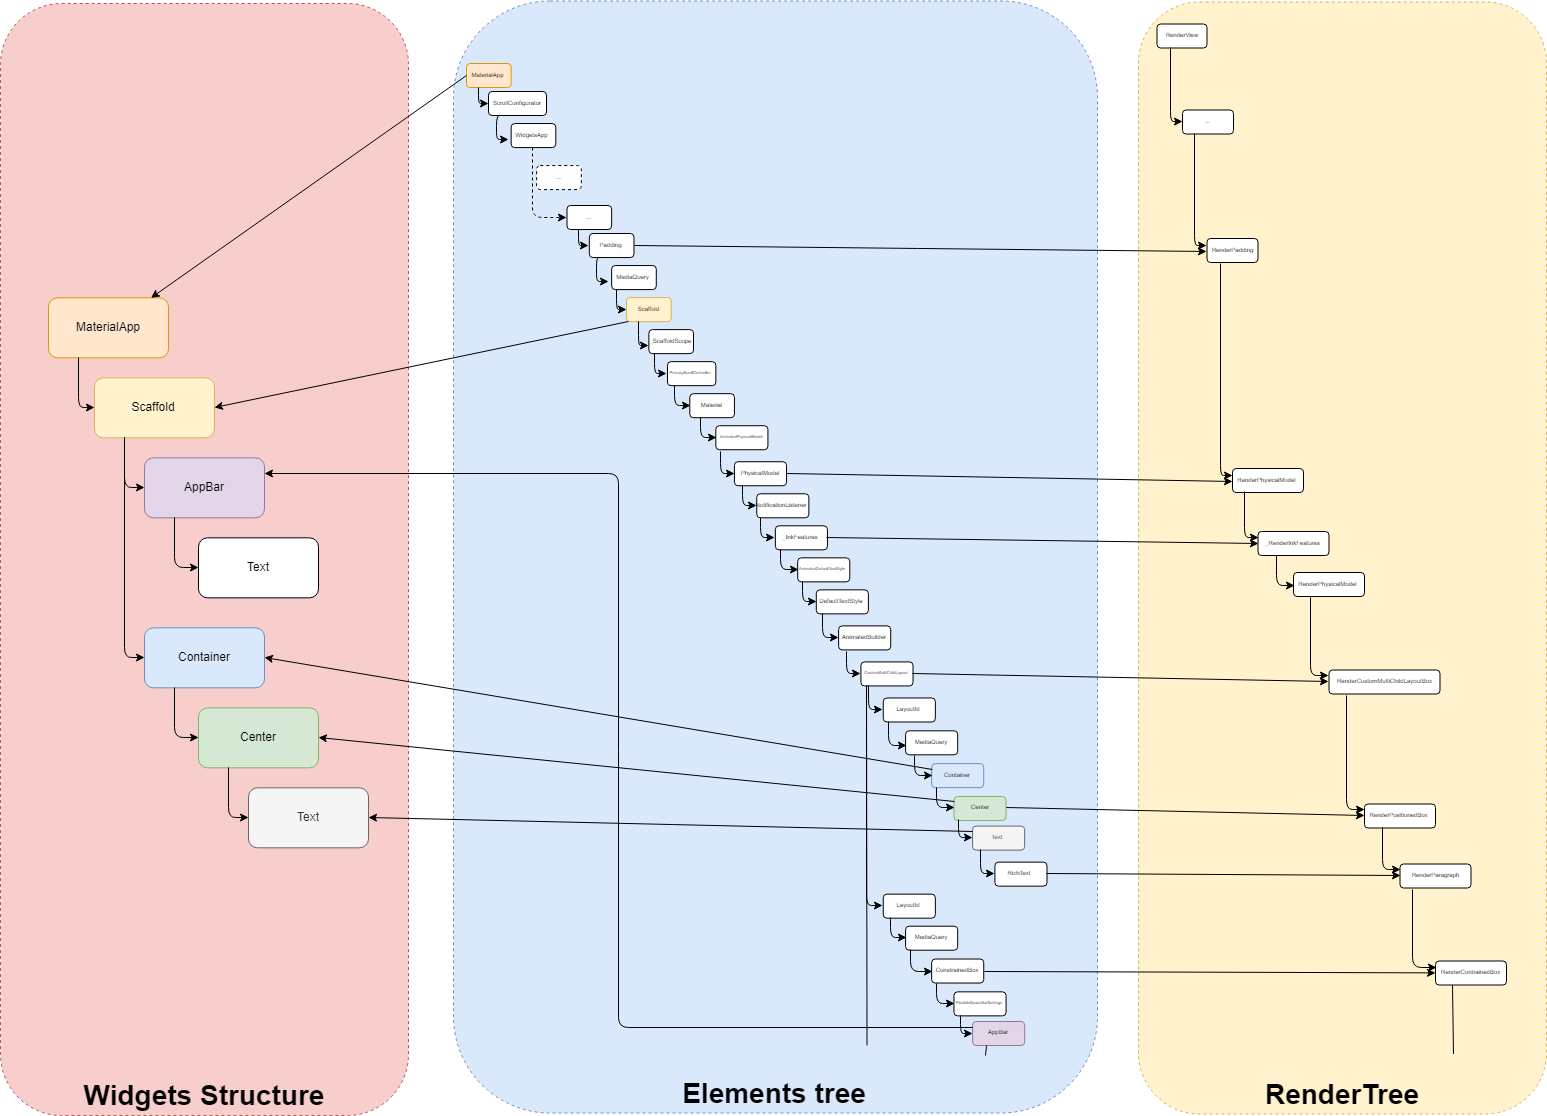
\includegraphics[width=0.75\linewidth]{img/flutter/internals_3_trees.png}
    \caption{Three Trees -- Widget, Element and Render Tree~\cite{didier-internals}.}
    \label{fig:flutter-internal-3-trees}
\end{figure}

When Flutter needs to render the current state to the screen, the engine will request to inflate all widgets~\cite{didier-internals}. This can be simplified as unpacking the ``box of boxes''. Each Widget internally uses more granulated, and low-level API's Widgets in order to precisely describe the layout. Furthermore, from a developers perspective, the widgets create Widget tree. In fact, internally each Widget has assigned \textit{Element} object which forms the \textit{Element Tree}.

Each Element points to Widget which created it, parent and potentially child Element and may also point to a RenderObject~\cite{didier-internals}.  \Cref{fig:flutter-internal-3-trees} shows notion of ``widget tree'', Element~Tree and Render~Tree.

Every Widget can be assigned to one of the three categories~\cite{didier-internals}:
\begin{enumerate}
\item \textbf{The proxies}  -- these Widgets hold information which needs to be available to other Widgets -- such as \verb|InheritedWidget|.
\item \textbf{The Renderer}s -- These Widgets define the layout of the screen, such as Row, Column, Padding, \ldots
\item \textbf{The Components} -- These Widgets provide final information related to how the piece of~\gls{ui} should look. An~example of such a Widget can be Text or RaisedButton. 
\end{enumerate}
Depending on the Widget category, a corresponding Element type is associated. There are two main Element types - \textit{ComponentElement} and \textit{RenderObjectElement}. The first one does not directly correspond to visual rendering. The latter one has a connection to RenderObjects.  Also, every Widget has its corresponding Element object, speaking of StatefulWidget has corresponding StatefulElement where the state is associated. This statement also implies that BuildContext is Element itself. 
% --- # --- # --- # --- # --- # --- # --- # --- # --- # --- # --- # --- # --- # --- # --- # --- # --- # --- #
\subsection{Deciding What to Redraw}
A redraw mechanic relies on invalidating either an Element or a RenderObject~\cite{didier-internals}.  Whenever the Widget should be rebuilt, the corresponding Element is marked as dirty. Invalidation of RenderObject can happen, for example, when changes to its dimension, position or geometry are made or when the Element tree is marked as dirty. When engine decides that new repaint should happen, it iterates over all invalidated (dirty) elements and request them to rebuild. Internally the rebuild works as~\cite{didier-internals}:
\begin{quote}
    \begin{enumerate}
    \item The corresponding Widget's build method is called which returns a new Widget.
    \item If the Element has no child, the~new Widget is inflated.
    \item Otherwise the new Widget is compared to the one referenced by the~child element and
        \begin{itemize}
        \item if they are same (same widget type and Key), the update is made and the child element in the~Element Tree is kept,
        \item if they are not same, the child element is unmounted (and discarded) and the new Widget is inflated.
        \end{itemize}
    \item The inflating of the Widget leads to creating a new element, which is inserted into the element tree as a new child of the Element. 
    \end{enumerate}
\end{quote}


After that, the ElementTree is considered as a stable and a similar process is made with Render Tree -- every RenderObject marked as dirty performs its layout (calculating dimension and geometry), every RenderObject marked to repaint is repainted. In the end, the device screen is redrawn. 
% --- # --- # --- # --- # --- # --- # --- # --- # --- # --- # --- # --- # --- # --- # --- # --- # --- # --- #
\subsection{Notion of Keys}
When comparing new Widget with current one within Element, the Element decides to rebuild when the Widget type and Key are different. A \textit{Key} is an object associated with a Widget. In the simplest form, a Key can be considered as the unique identification of the Widget. In most cases, developers should not need to work with the keys as Flutter manage them internally. However, there are cases where the manual definition of the Key is necessary. 

\begin{figure}[ht]
    \centering
    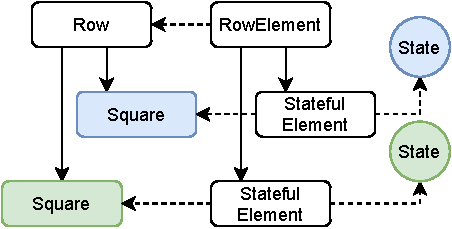
\includegraphics[width=0.75\linewidth]{img/flutter/key_stateful_start.pdf}
    \caption{Square Widgets and Associated Elements with States.}
    \label{fig:keys_start}
\end{figure}

\begin{figure}[ht]
    \centering
    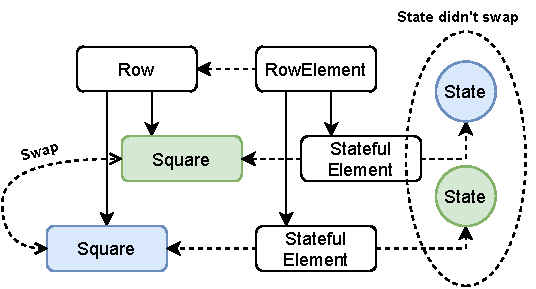
\includegraphics[width=0.75\linewidth]{img/flutter/key_stateful_wrong_state.pdf}
    \caption{Square Widgets After Swap and Associated Elements With Wrong States.}
    \label{fig:keys_wrong}
\end{figure}

\begin{listing}[ht]
\begin{minted}{dart}
// SquarePage holds list of Square widgets
class _SquaresPageState extends State<SquaresPage> {
  final squares = [Square(RandomColor.get()), 
                    Square(RandomColor.get())];
  void _shiftSquares() {
    setState(() => squares.insert(1, squares.removeAt(0)));
  }

  @override
  Widget build(BuildContext context) {
    return Scaffold(
        body: Row(children: squares),
        floatingActionButton: FloatingActionButton(
          onPressed: _shiftSquares,
          //...
        ),
      );
   }
}
\end{minted}
\caption{SquarePage Widget With Stateless Square Widgets.}
\label{listing:keys_page_stateless}
\end{listing}

The problem can occur when some Widget uses a collection of Widgets of the~same type that holds some state.  Consider a concrete example where \verb|SquarePage| holds a list of \verb|Square| widgets~(\Cref{listing:keys_page_stateless}). Each \verb|Square| (as a StatelessWidget) has defined random colour through a constructor. After a~button is clicked, the squares are swapped. With \verb|Square| as StatelessWidgets, everything works as expected. 

\begin{listing}[ht]
\begin{minted}{dart}
class Square extends StatefulWidget {
  Square({Key key}) : super(key: key);
  @override
  _SquareState createState() => _SquareState();
}

class _SquareState extends State<Square> {
  Color color;
  @override
  void initState() {
    color = RandomColor.get();
  }

  @override
  Widget build(BuildContext context) {
    return Container(color: color,width: 100,height: 100);
  }
}
\end{minted}
\caption{Square Widget as StatefulWidget.}
\label{listing:keys_square_stateful}
\end{listing}

However, if the~\verb|Square| becomes StatefulWidget~(\Cref{listing:keys_square_stateful}) and the button is clicked, it seems like nothing happened -- squares stay on the same place. As was said when the~Widget is marked to rebuilt, it walks through Elements and if the Widget type and the Key match the Element updates its reference to new Widget. In the~case of StatefulWidget, the associated state is linked to the~Element object~(\Cref{fig:keys_start}). When squares are shifted, the~Element is marked as dirty. It walks through square's StatefulElement and checks if Widget type and Key matches -- and they are as no Keys are assigned. Hence, the~Element updates its Widget reference, but the~associated state remains the~same~(\Cref{fig:keys_wrong}). 
The key is to add Key. There are several types of Keys such as ValueKey, where some unique value can be assigned (for example article's id). For \verb|Square| example, the \textit{UniqueKey} which generates unique identification is enough.  After the Keys are assigned, \mint{dart}|final squares = [Square(key: UniqueKey()),Square(key: UniqueKey())]| the example works again as expected. The~full example code is available as~before within appendix.

The keys should be put to the most top Widget, which is used as a root widget of collection. Otherwise, the rebuilding algorithm fails once again, and wrong behaviour will occur. In practice, Key should be used when stateful widgets are used within collections (such as ListView, Row or Column) and they are manipulated -- moved, removed and similar.  Moreover, sometimes the GlobalKey can be used to manage some Widget's state ``outside''. This approach is often used with managing text inputs. 
% --- # --- # --- # --- # --- # --- # --- # --- # --- # --- # --- # --- # --- # --- # --- # --- # --- # --- #
\subsection{Const Optimisation}
On of the Dart's features are \textit{const} constructors which makes instance as a~\textit{compile-time constant}. This feature can be used to optimise widget builds and prevent unnecessary rebuilds. Most of the Widgets has \textit{const} constructor, and if possible, the~\textit{const} constructor should be used. Such as Icon widget or Text widget if they accept non-changing values they can be made compile-time constants and Flutter when rebuilding the tree will these Widget reuses instead of creating a new one. 

The problem of performance optimisation is a vast subject for discussion, and it could have its own chapter. The~const constructors are only ``tip of the iceberg''. In general, it is somewhat common sense to~avoid unnecessary \gls{ui} rebuilds or avoid using animations carelessly such as animate each line of Text within ListView whenever the~list is updated. Some other optimisation tips are discussed later in the~implementation chapter. 

\section{Conclusion}
The first chapter introduced Flutter framework and its philosophy ``everything is a widget'' as a~primary user interface building block. The~notion of state and several state management approaches were discussed, how they can be implemented and how they affect the rebuilding of~\gls{ui}. In the~end, part of Flutter internals was uncovered and explained to grasp a better understanding of how the~framework works.

\chapter{Coffee Time Analysis}
\label{ch:analysis}
In this chapter, the specification of the implemented application is outlined. The analysis of similar applications was made to obtain ideas.  After analysis, the low fidelity prototype was created to outline the first vision of the final application. Next, the high-fidelity prototype, along with Nielsen's heuristics analysis and user testing, were made. At the end of the chapter, considered tools and services which are used to implement the application are briefly described. 
% ----- % ----- % ----- % ----- % ----- % ----- % ----- % ----- % ----- % ----- % ----- % ----- % ----- % ----- %
\section{Considered Application}
Coffee Time is an application focused on searching nearby cafes. Users should be able to search and find nearby cafes around them and decide which establishment to visit. Each cafe is displayed with information such as distance, user's reviews, photos, opening hours and more. 

Added value to this standard information is a feature so-called ``the tags''. These tags are user-added additional info which describes more precisely what given cafe offer or for instance if that cafe allows pets inside. 

The set of tags is defined, and users can add these tags to the~cafe.  Each tag can be reviewed by other users. These reviews are done through ``like'' and ``dislike'' functionality. The~purpose of tag's reviews is to prevent outdated information or misleading information.  

The example of such review can be ``User visited cafe which has tag 'dog friendly', but unfortunately this information was incorrect. Consequently, the~user decided to open the~application and review the~cafe's tag 'dog friendly' with dislike.''

Together with likes and dislikes, each tag has a computed score.  Each like gives to score plus one and as an opposite, dislike minus one. 
If any tags reach the score to~-4, the~tag is removed from the cafe, more precisely is not shown anymore to users. 
If such removed tag is proposed by any user again, it obtains ``like'' review. Thus score is incremented to -3 and the tag is shown again. 

The application is location-based and offers a map view to support the~convenient user experience. Any cafe can be marked as user's favourite to~give a faster way to find cafe whenever the user wants. 

In conclusion, Coffee Time is application focused on one domain -- searching nearby cafes in order to know where to~go to~study, talk with friends or~for example have a great coffee. The application should be simple to use with a clean user interface. 
% ----- % ----- % ----- % ----- % ----- % ----- % ----- % ----- % ----- % ----- % ----- % ----- % ----- % ----- %
\section{Use Cases}
From the specification above, the use cases and use case scenarios were formed. The~use cases diagram is listed in \Cref{fig:use_case} and shows every use cases from the~user perspective. Technically there is the role of application administrator who can check control back-end or available application's tags, but it is skipped due to the lack of importance from application perspective. 

\begin{figure}[htp]
    \centering
    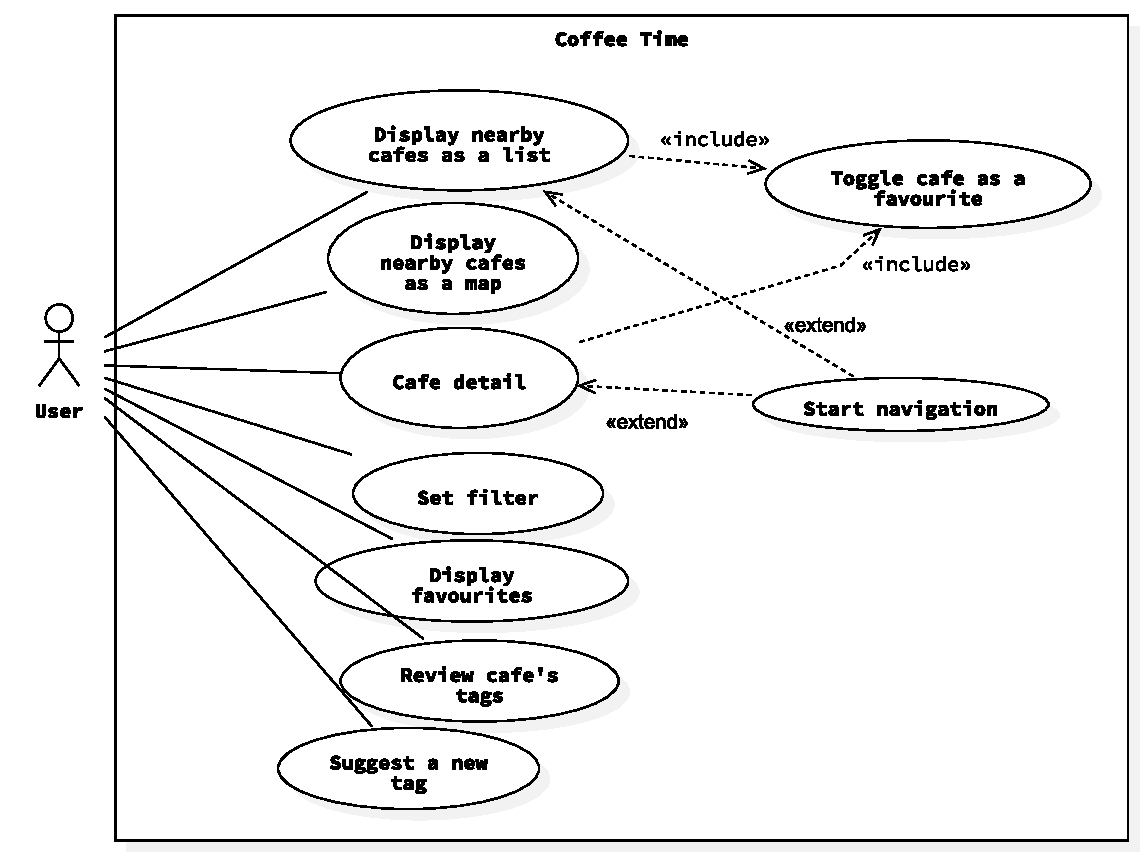
\includegraphics[width=\linewidth]{img/analysis/use_case.pdf}
    \caption{Application's use case diagram}
    \label{fig:use_case}
\end{figure}

As shown on diagram, the application has several use cases listed below

\begin{itemize}
    \item UC1: Display nearby cafes as a list.
    \item UC2: Display nearby cafes as a map.
    \item UC3: Start navigation.
    \item UC4: Toggle cafe as a favourite.
    \item UC5: Setting the filter.
    \item UC6: Display favourite cafes.
    \item UC7: Review the cafe's tags.
    \item UC8: Suggest a new tag.
\end{itemize}

\subsection{UC1: Display Nearby Cafes As a List}
User can display nearby cafes in the form of the list view. The result is filtered by setting a filter, which can be altered by \textit{UC5}.

\newpara
\noindent \textbf{Pre-Conditions} The user must be on the cafe list screen.

\newpara
\noindent \textbf{Basic Flow}

\begin{enumerate}
    \item User launch Coffee Time and lands on cafe list.
    \item Cafe list shows nearby cafes around him. Each cafe is displayed in the form of a card.
    \item User can pull the list down to refresh results. 
    \item User taps on cafe's card and is redirected to the detail view.
\end{enumerate}

\noindent \textbf{Alternative Flow 1} The user launch navigation to the selected cafe.

% -------------

\subsection{UC2: Display Nearby Cafes as Map}
User can display nearby cafes in the form of the map view. Each cafe is shown as a map marker.
\newpara
\noindent  \textbf{Pre-Conditions} The user must be on the map screen.

\newpara
\noindent \textbf{Basic Flow}

\begin{enumerate}
    \item User launch application and change screen to map view. 
    \item Nearby cafes are shown as markers.
    \item The user taps on the marker and is redirected to the detail screen.
\end{enumerate}

\noindent  \textbf{Alternative Flow 1} The user taps anywhere on the map to display nearby cafes on the selected location.

% -------------

\subsection{UC3: Start navigation}
This use case allows starting navigation to selected cafe through native navigation applications.
\newpara
\noindent \textbf{Pre-Conditions} The navigation services must be enabled.

\newpara
\noindent \textbf{Basic Flow}

\begin{enumerate}
    \item The user selects the cafe.
    \item The user selects navigate action. 
    \item The system request to open navigation application is opened. 
    \item User enables navigation and is redirected to navigation application. 
\end{enumerate}

\noindent \textbf{Alternative Flow 1} The user dismisses navigation request and cancels navigation.

% -------------
\subsection{UC4: Toggle cafe as a favourite}
Each cafe can be marked as a favourite to faster future access. 

\newpara
\noindent \textbf{Pre-Conditions} The cafe must be loaded, so that it is visible to the~user. The~user must be either on the~cafe list screen, detail screen or favourite screen. 

\newpara
\noindent \textbf{Basic Flow}

\begin{enumerate}
    \item User has a cafe which wants to toggle as a favourite.
    \item User toggles cafe as a favourite.
\end{enumerate}

% -------------

\subsection{UC5: Setting the filter}
User changes the filter settings to filter out the cafe results.

\newpara
\noindent \textbf{Pre-Conditions} There are results to filter.

\newpara
\noindent \textbf{Basic Flow}

\begin{enumerate}
    \item User opens filter settings screen.
    \item If it is suitable user changes results ordering from ``by distance'' (default) to ``by popularity''.
    \item If it is suitable user changes opening hours filter.
    \item Add tags to filter by, if any.  
    \item Returns back to the previous screen
    \item The results are filtered with the chosen filter.
\end{enumerate}

% -------------

\subsection{UC6: Display favourite cafes}
Display every favourite cafe in the form of the list view. 

\newpara
\noindent \textbf{Pre-Conditions} The user must be on the map screen.

\newpara
\noindent \textbf{Basic Flow}

\begin{enumerate}
    \item User displays favourite cafe list.
    \item After the cafe is selected, the user is redirected to the cafe's detail screen.
\end{enumerate}

\textbf{Alternative Flow 1} The user launches navigation to the selected cafe.

\textbf{Alternative Flow 2} The user toggles cafe as not-favourite anymore.

% -------------

\subsection{UC7: Review the cafe's tags}
Use case allows users to review the cafe's tags with likes and dislikes. 

\newpara
\noindent \textbf{Pre-Conditions} Cafe must have tags to review.  User must be on the cafe's detail screen.

\newpara
\noindent \textbf{Basic Flow}

\begin{enumerate}
    \item The user wants to suggest a change to the selected cafe.
    \item User reviews each tag with 'like', 'dislike' or skip review for the given tag. 
    \item User confirms review.
\end{enumerate}

\noindent \textbf{Alternative Flow 1} The user decides not to do the review and goes back to the detail screen.

% -------------

\subsection{UC8:  Suggest a new tag}
Use case allows users to suggest a new tag to the selected cafe.

\newpara
\noindent \textbf{Pre-Conditions} Cafe must have tags to review.  User must be on the cafe's detail screen.

\newpara
\noindent \textbf{Basic Flow}

\begin{enumerate}
    \item The user wants to suggest a change to the selected cafe.
    \item The user selects new tags for the suggestion. 
    \item The user confirms the suggestion.
\end{enumerate}

\noindent \textbf{Alternative Flow 1} The user decides not to make the suggestion and goes back to the detail screen.

% -------------

\section{Existing Alternatives}
The analysis of existing alternatives was made to research already created applications with similar features. Existing applications were searched through Android's official store. Applications with these functionalities were chosen for the review:

\begin{itemize}
    \item nearby place search,
    \item application's theme should be cafes or similar.
\end{itemize}

For comparison the most five inspiring and distinguish applications were chosen. The following lines briefly describe one of each, their target audience, the advantages and drawbacks. 

\subsection{Gastromapa Lukáše Hejlíka}
Published in the first quarter of 2019 as a new application for exploring restaurants in the Czech Republic. The application's speciality is that restaurants' reviews are not done by users but by gastronomy specialist \textit{Lukáš~Hejlík}.

As soon as the application launches, it displays nearby restaurants. Each establishment is shown as a card with important information such as an address, distance, and type of restaurant. The main card's focus is a large photo which should catch the user's eye to take a look. 

After the card is clicked, the user is presented with the restaurant's detail, where more information such as opening hours, map location and comprehensive review by~\textit{L.~Hejlík} can be found. From this detail navigation to the chosen restaurant can be launched. The target audience is anyone who seeks to visit unknown places and possess the opportunity to taste great food.

\begin{figure}[ht]
    \centering
    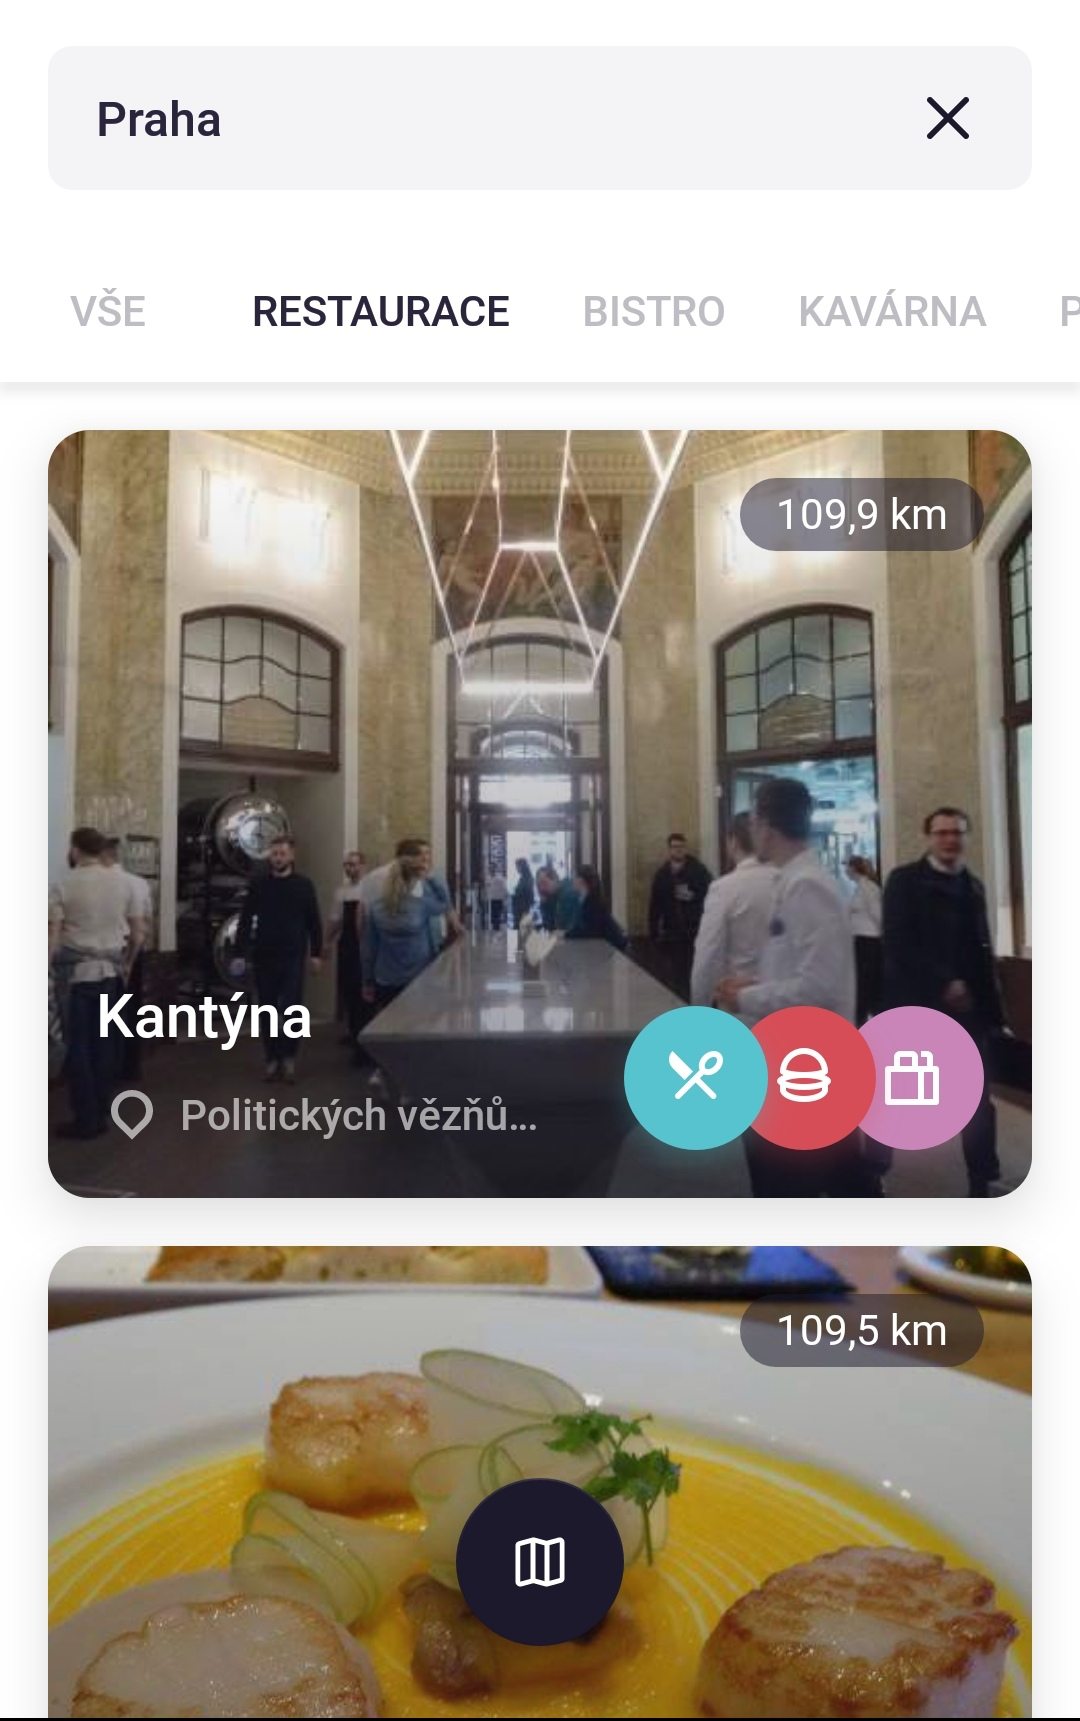
\includegraphics[width=0.33\linewidth]{img/analysis/app-hejlik.jpg}
    \caption{Gastromapa \textit{L. Hejlíka} \cite{app-hejlik}}
    \label{fig:gastromapa-hejlik}
\end{figure}

\subsubsection{The advantages}
\begin{itemize}
    \item Design is fresh, clean and users can immediately see relevant content.
    \item Thanks to clean design application is easy to use and understand.
    \item The whole application behaves smoothly without any noticeable freezing.
\end{itemize}

\subsubsection{The drawbacks}
\begin{itemize}
    \item The navigation button has a blackish colour that after scrolling disappears. If the restaurant has a darker photo, the button is hard to notice. 
    \item When coming back to the main screen, loading of the list is started again, and the previous search is lost.
    \item Detail screen on entry is fully covered with restaurant photo. From a design point of view, it is a nice touch, but users must scroll to see any information. 
\end{itemize}

\subsection{Pivní deník}
Application \textit{Pivní deník} is used to search nearby pubs in the Czech Republic and their beer offer. The content is created by the community, including served beer and their prices.  Application offers searching nearby restaurants filtered by beer brands. Each user can view a history of places they have visited. Furthermore they can mark any pub as their favourite and share their experience.


\begin{figure}[ht]
    \centering
    \begin{minipage}{0.45\linewidth}
        \centering
        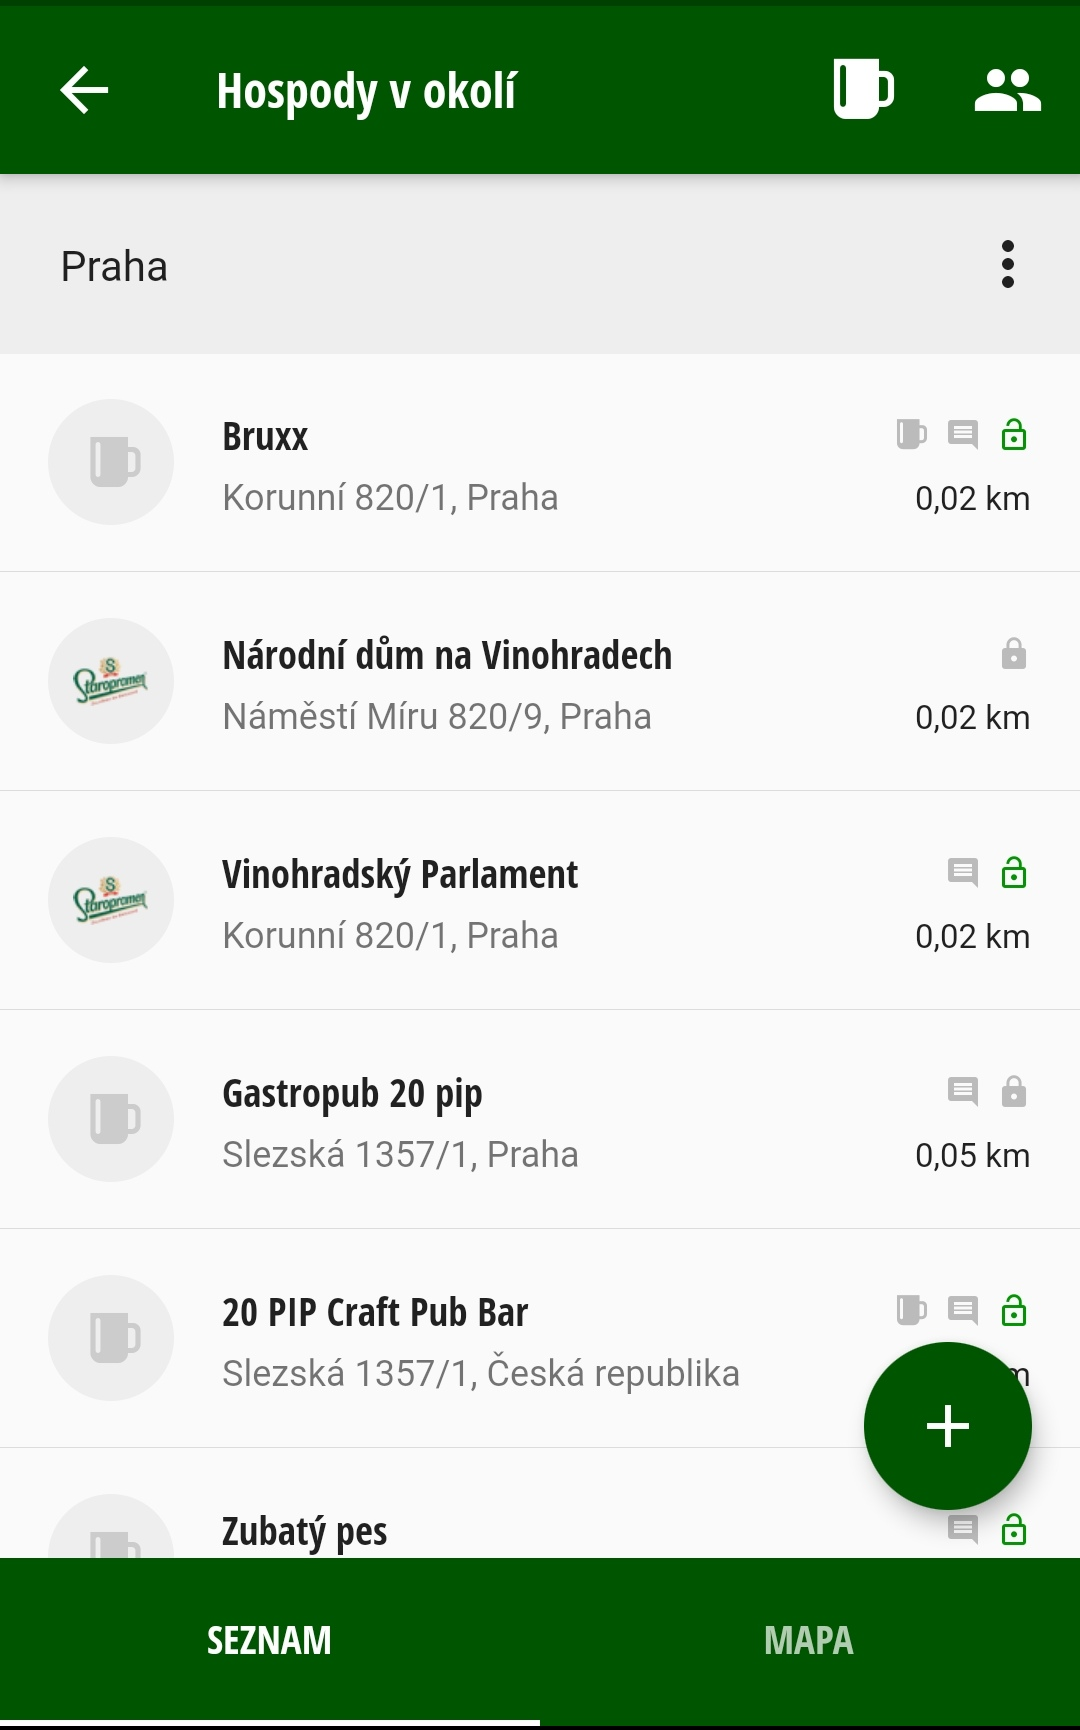
\includegraphics[width=0.75\linewidth]{img/analysis/app-pivni-denik.jpg}
        \caption{Pivní deník \cite{app-pivni-denik}}
        \label{fig:pivni-denik}
    \end{minipage}\hfill
    \begin{minipage}{0.45\linewidth}
        \centering
        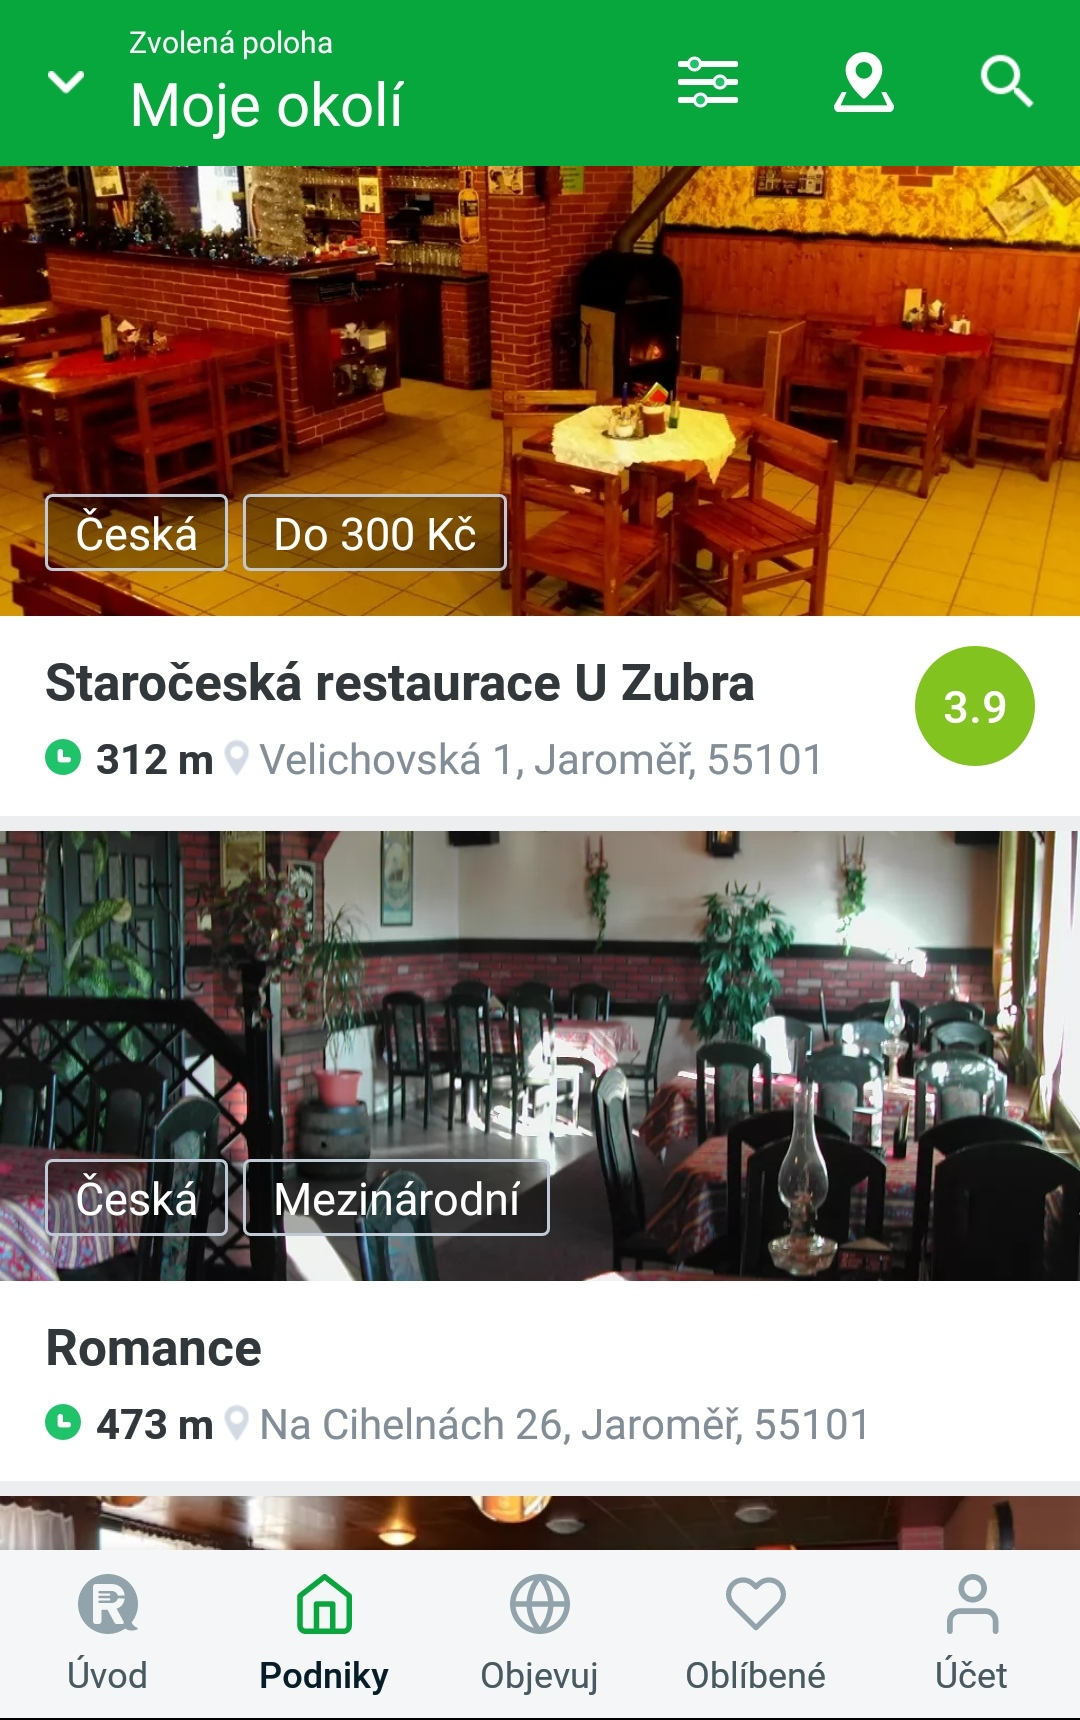
\includegraphics[width=0.75\linewidth]{img/analysis/app-restu.jpg}
        \caption{Restu \cite{app-restu}}
        \label{fig:restu}
    \end{minipage}
\end{figure}

% \begin{figure}[ht]
%     \centering
%     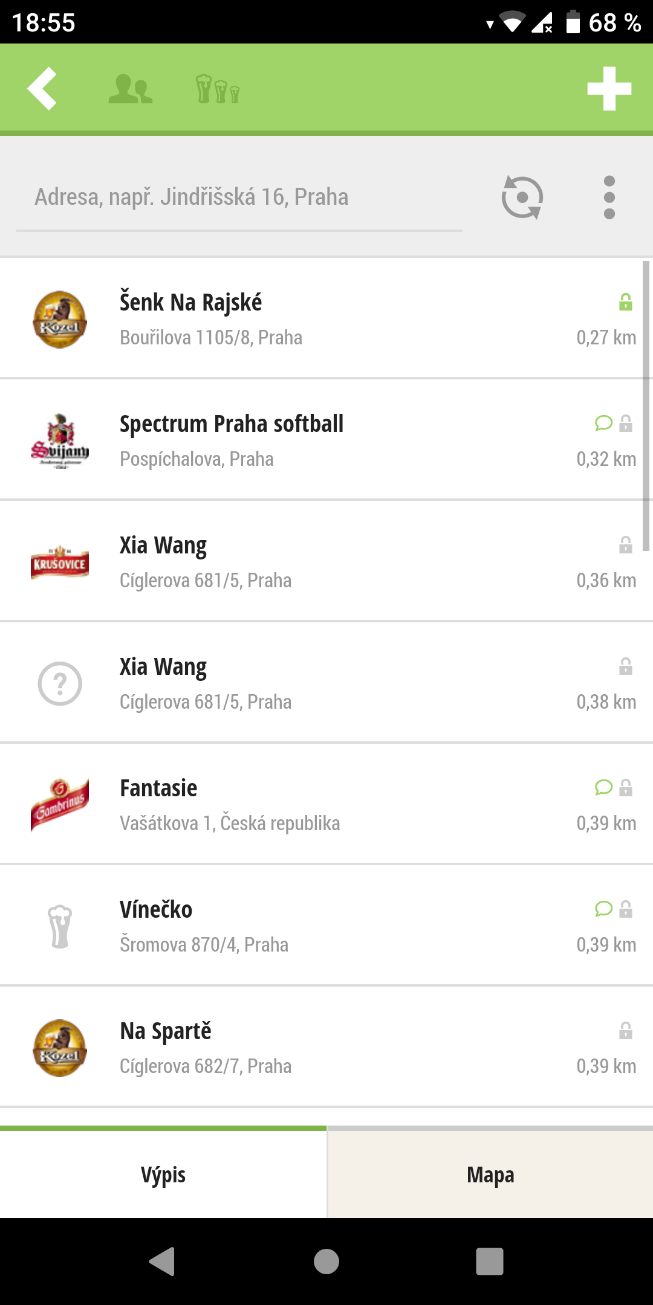
\includegraphics[width=0.25\linewidth]{img/analysis/pivni_denik.png}
%     \caption{Pivní deník \cite{app-pivni-denik}}
%     \label{fig:pivni-denik}
% \end{figure}

\subsubsection{The advantages}
\begin{itemize}
    \item Pubs are displayed as a list or points on the map.
    \item The served brands are displayed directly within the list, so it is not needed to visit details.
    \item The registration is optional for searching. If users want to contribute, they have to have an account.
\end{itemize}

\subsubsection{The drawbacks}
\begin{itemize}
    \item A registration can be done through Facebook or e-mail. With e-mail registration, the user is forced to leave the application and is redirected to the web page where registration is finished.
    \item As was said, content is created by the community. During the research, it was clear that many information is outdated or misleading. 
    \item Overall the application design looks outdated and does not meet current, modern, trends.
    \item On the primary screen, there are displayed user's stats and the most three nearest pubs. The~drawback is that on the~larger screens, there is plenty of unused space. 
    \item Each restaurant displays only one brand of drafted beer. Nowadays, many pubs offer more than one brand. 
    \item The side menu can be opened only with the hamburger icon but not with slide to the right gesture.
\end{itemize}

\subsection{Restu}
\textit{Restu} is another gastronomy guide focused on restaurants in the Czech Republic. Through this application reservations can be made. Application has many unique functionalities. For example ``discover'' section which shows attractive offers or the best cafe in the city. Another functionality is the ``check-in'' button which gives credits to the users if they eat at the~given restaurant. Target audience is everyone who searches for new places where to eat and make a~reservation.

% \begin{figure}[ht]
%     \centering
%     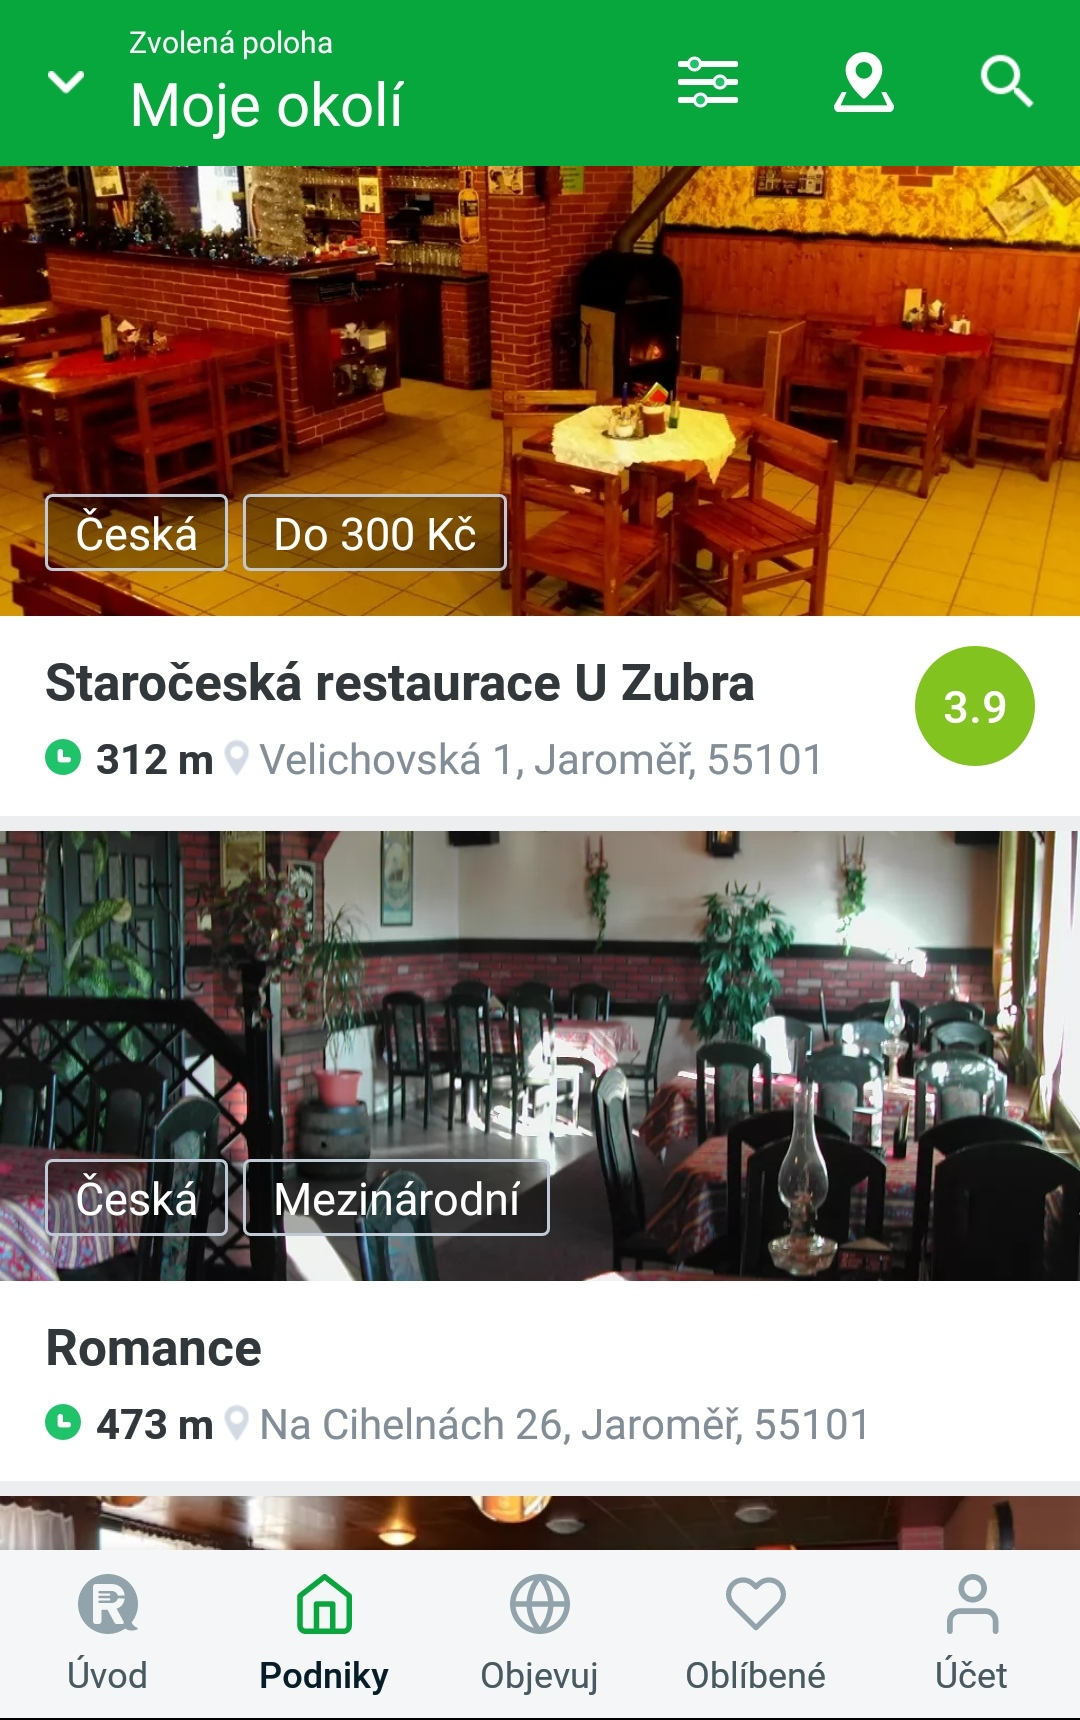
\includegraphics[width=0.33\linewidth]{img/analysis/restu.jpg}
%     \caption{Restu \cite{app-restu}}
%     \label{fig:restu}
% \end{figure}

\subsubsection{The advantages}
\begin{itemize}
    \item Clean and well-structured layout.
    \item Opt-in registration.
\end{itemize}

\subsubsection{The drawbacks}
\begin{itemize}
    \item When a restaurant card is selected, window of the restaurant pops up but at the bottom cannot be hidden again.
    \item To review the restaurant, the user has to be signed in and the restaurant must be open. If the restaurant is closed, the review cannot be added.
\end{itemize}

\subsection{Zomato}
\textit{Zomato} is primarily web-based restaurant browser in the world. It has its own database of establishments. Content is edited by users.  
On the primary screen there are displayed ``week hits'', top restaurants, or ``happy hours''. Restaurants are divided into categories such as ``Nightlife'' or ``Daily menu'' which helps for navigation within the application.
Target audience is anyone who wants to try new restaurants or someone who is looking for action offers.

% \begin{figure}[ht]
%     \centering
%     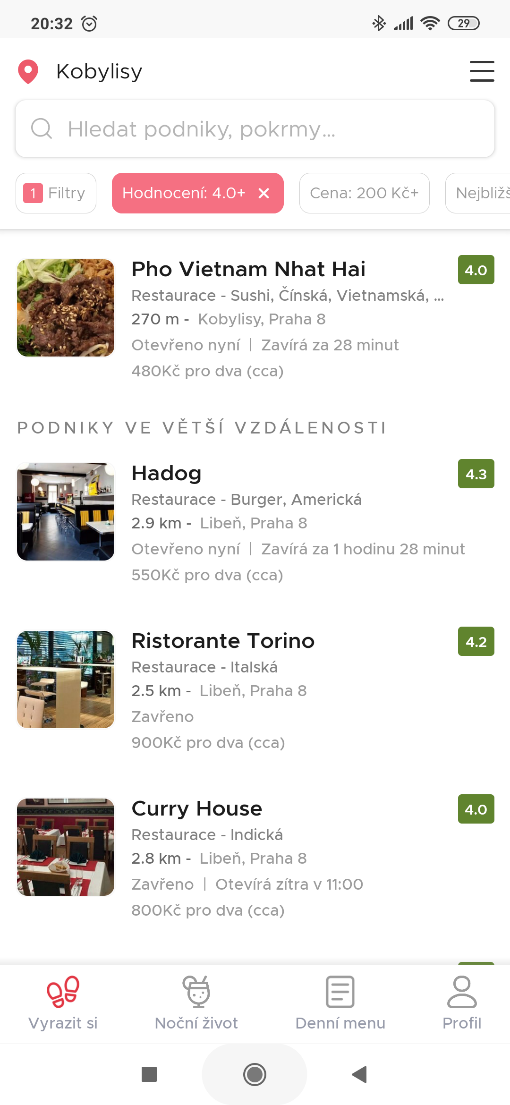
\includegraphics[width=0.33\linewidth]{img/analysis/zomato.png}
%     \caption{Zomato \cite{app-zomato}}
%     \label{fig:zomato}
% \end{figure}

\begin{figure}[ht]
    \centering
    \begin{minipage}{0.45\linewidth}
       \centering
    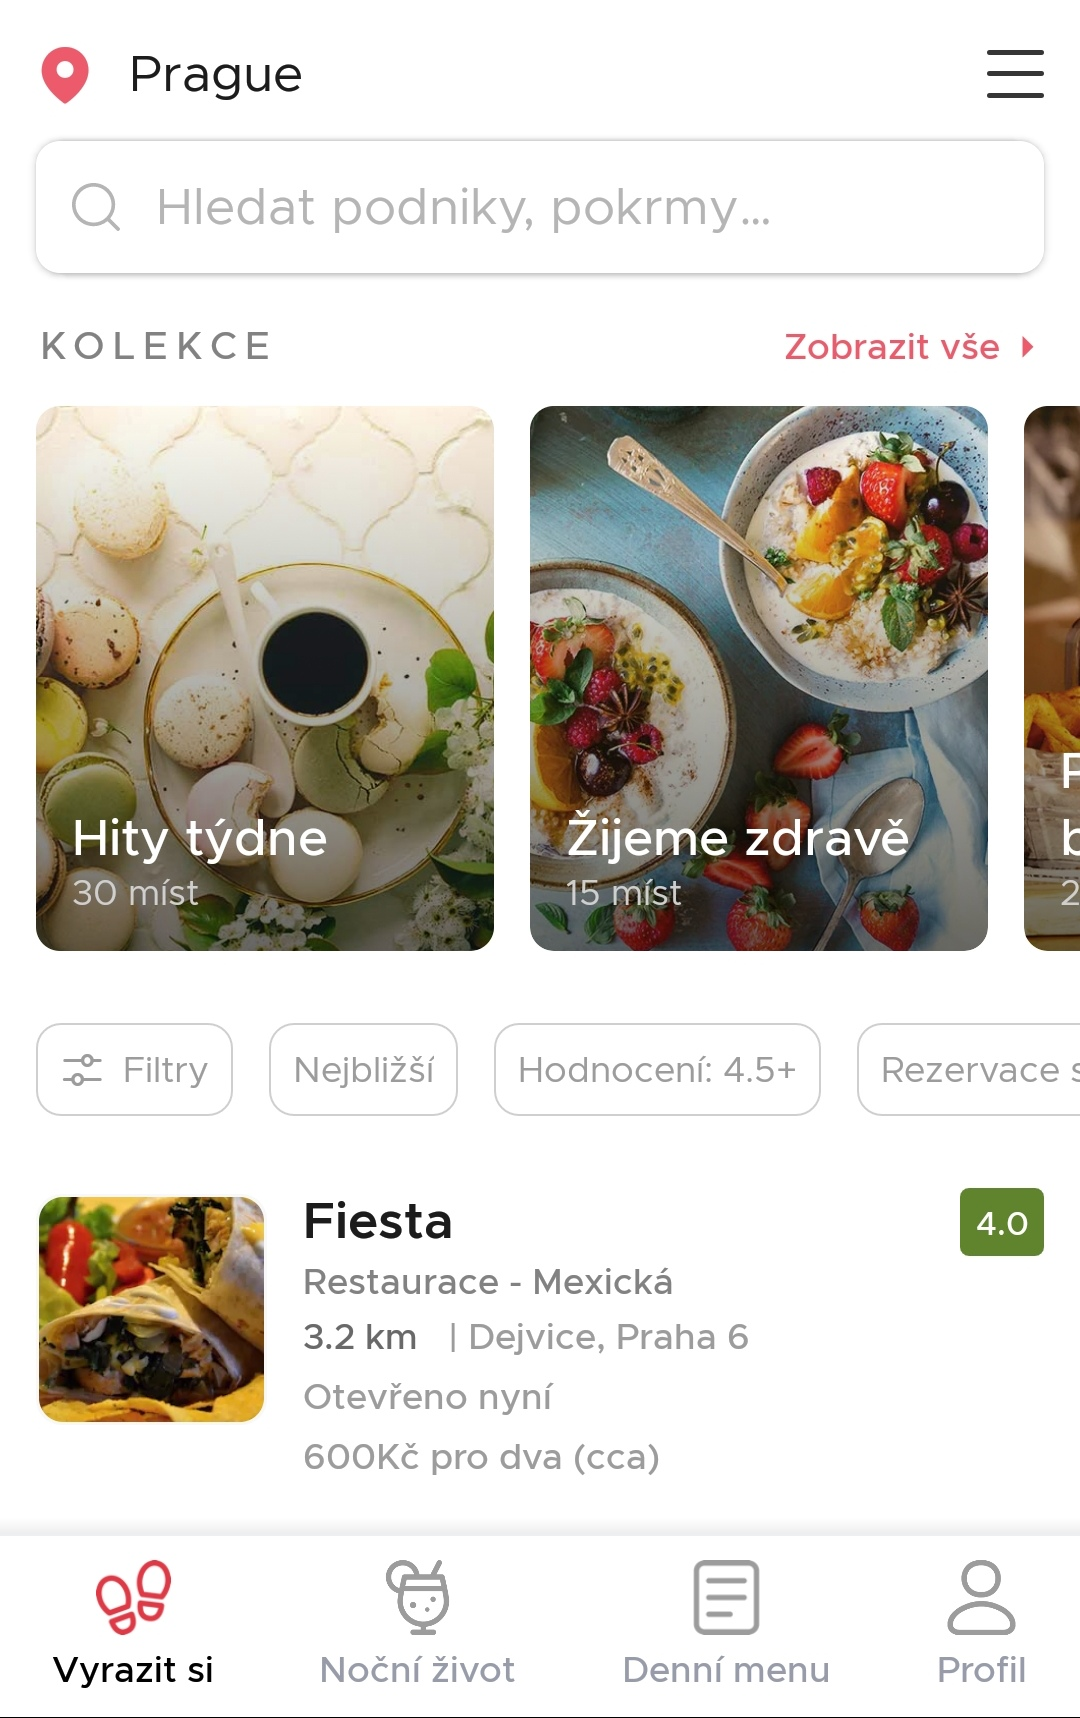
\includegraphics[width=0.75\linewidth]{img/analysis/app-zomato.jpg}
    \caption{Zomato \cite{app-zomato}}
    \label{fig:zomato}
    \end{minipage}\hfill
    \begin{minipage}{0.45\linewidth}
        \centering
        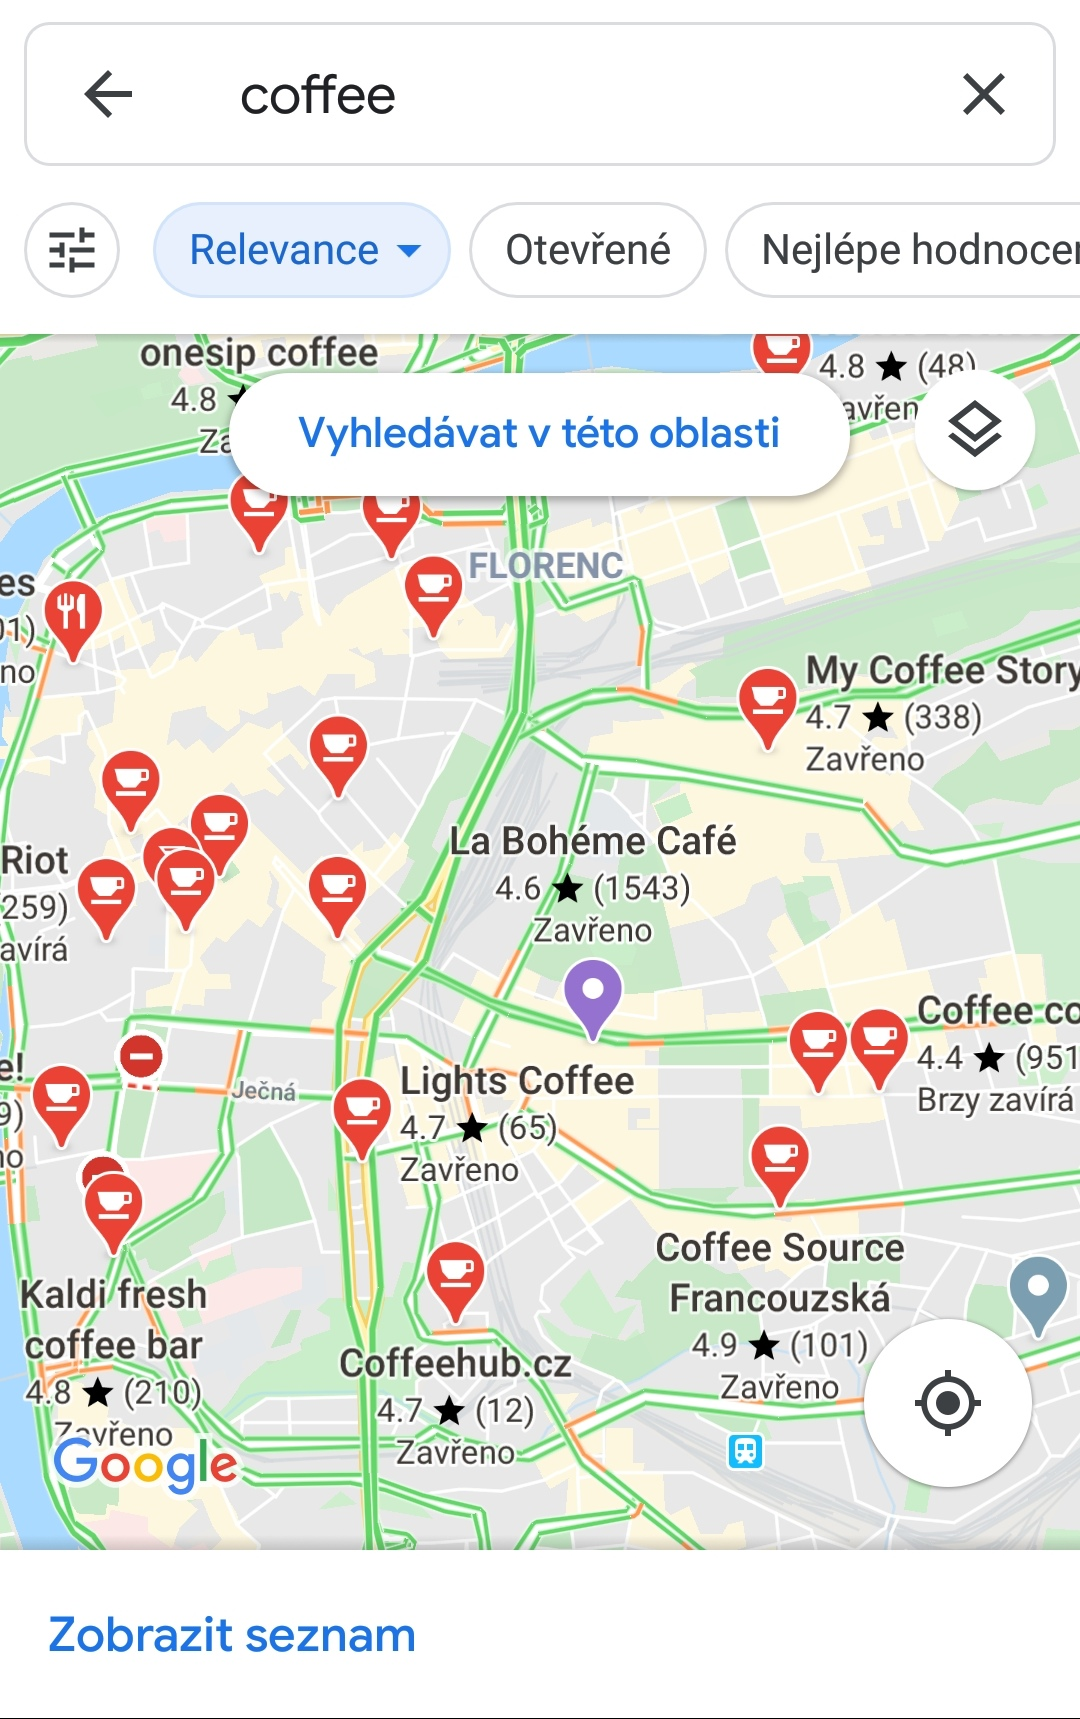
\includegraphics[width=0.75\linewidth]{img/analysis/app-gmaps.jpg}
        \caption{Google Maps \cite{app-google-maps}}
        \label{fig:google-maps}
    \end{minipage}
\end{figure}

\subsubsection{The advantages}
\begin{itemize}
    \item Well solved filtering. The filter setting is intuitive and it displays the most used filters. 
    \item Advanced options for filtering with tags such as ``dog friendly'' or ``Wi-Fi free''.
    \item Friendships with other users. If another user added a~review, notification is received.
\end{itemize}

\subsubsection{The drawbacks}
\begin{itemize}
    \item The primary screen is cluttered with many information at one place.
    \item Nearby restaurants list is hidden below ``favourites restaurants'' and ``month collections''.
    \item The full-text search in some circumstances behaves unexpectedly. For example, to search for restaurants which offer ``Asian food'' user has to type exactly ``asian'' but not ``asia''.
    \item Readability of some text is worsened by light background and greyish text colour. In some scenarios, it is hard to read the content.
\end{itemize}

\subsection{Google maps}
Popular worldwide map service by \textit{Google}. One of the world's biggest database of places, including restaurants. 
\textit{Google maps} for each business, establishment displays additional info such as user reviews, photos, prices. 
Within Android system is already installed. Nearby places can be searched directly from the map.

% \begin{figure}[ht]
%     \centering
%     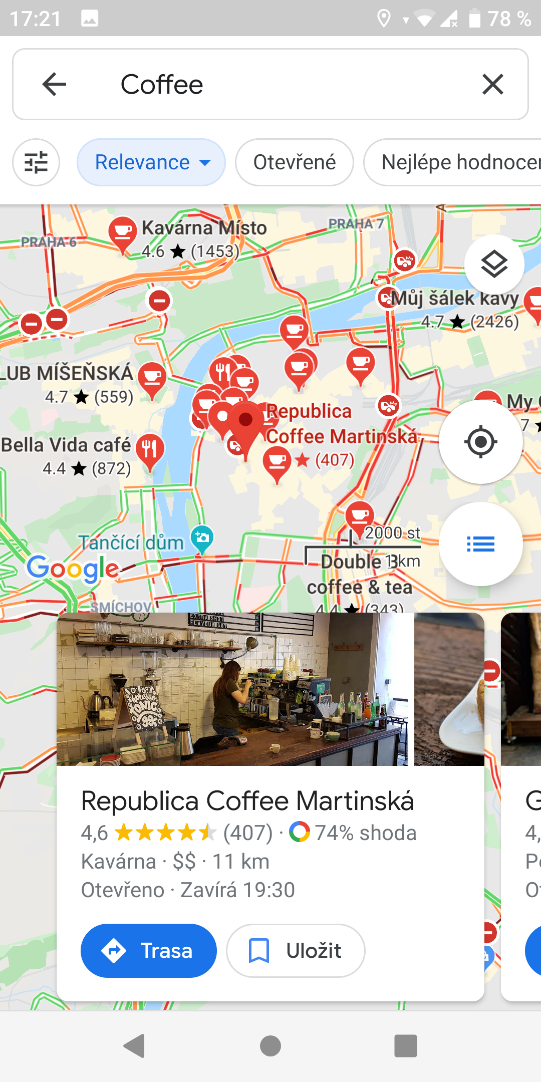
\includegraphics[width=0.33\linewidth]{img/analysis/gmaps.png}
%     \caption{Google Maps \cite{app-google-maps}}
%     \label{fig:google-maps}
% \end{figure}

\subsubsection{The advantages}
\begin{itemize}
    \item Well known and tested user interface which is embedded often to another application.
    \item No registration is required.
    \item A place detail includes plenty of useful information.
    \item GPS navigation with one click.
\end{itemize}

\subsubsection{The drawbacks}
\begin{itemize}
    \item Not domain focused, that means it does not offer focused content on particular businesses such as restaurants.
    \item No advanced filtering and result sorting.
\end{itemize}

In conclusion, five applications were analysed on the Android system. Three apps are focused mainly on gastronomy. Another one specialises on beer. Last one, \textit{Google maps} is one of the most universal and robust. 
Each application has its own unique \gls{ui} and overall user experience differs. In ~\Cref{table:app-analysis} the~targeted audience and user interface usefulness is summarised.

\begin{table}[htbp]
\centering
\begin{tabular}{|l|l|l|}
\hline
\multicolumn{1}{|c|}{Application} & \multicolumn{1}{c|}{Targeted audience} & \multicolumn{1}{c|}{Overall \gls{ui}} \\ \hline
Gastromapa Lukáše hejlíka         & Everyone                               & Great                           \\ \hline
Pivní deník                       & Beer drinkers                          & Bad                            \\ \hline
Restu                             & Everyone                               & Bad                            \\ \hline
Zomato                            & Everyone                               & Good                            \\ \hline
Google                            & Everyone                               & Great but complex              \\ \hline
\end{tabular}
\caption{Analysed applications \gls{ui} summarization}
\label{table:app-analysis}
\end{table}

% ----- % ----- % ----- % ----- % ----- % ----- % ----- % ----- % ----- % ----- % ----- % ----- % ----- % ----- %
\section{Application Prototype}
One crucial step during the creation of software product is prototyping. Prototypes can help introduce different design ideas, can be easily tested, evaluated and changed. Prototyping techniques differ, but the desired output is the same -- provide visually concept of the final product. Prototypes do not help only visually, but they are part of user experience research and can find out which parts of the user interface should be changed before it is implemented.

There is no correct definition of how prototypes should look like and how they should be created. The~prototype can be made from the form of a simple sketch on paper to sophisticated pixel-perfect application~\cite{adobe-prototype}. Prototypes can be created multiple times during the whole creation process. 

In the early stages, \gls{lofi} prototype is typically created. With \gls{lofi}, the application can be evaluated and user-tested if desired design concept is usable and understandable for users. When \gls{lofi} is finalised, the next prototype~--~\gls{hifi} is created. \gls{hifi} comes out from \gls{lofi} and should behave as fully functional application on the target platform. With \gls{hifi} once again, the application is evaluated with users and tested. 

To be more precise, according to \cite{adobe-prototype}, \gls{lofi} prototype is a~way to translate high-level concepts into tangible and testable artefacts. The most significant  functionality of \gls{lofi} prototypes is to check and test the functionality of the~product before visual appearance. Advantage of \gls{lofi} is that it is inexpensive, fast way to propose prototype. On the other hand, \gls{lofi} lacks complexity and cannot supply advanced interactivity. \gls{lofi} should be used to quickly create a prototype and get user feedback in the early stages of the creation process. 

After the~\gls{lofi} prototype, the \gls{hifi} is created. This prototype appears and function as similar as possible to the actual built application. \gls{hifi} should be created on the targeted platform and behave as it is the~final product. The goal is to have more complex \gls{ui} interactivity and have better feedback from user testing. Thanks to the fact that prototype looks like a real application, user behaves more naturally and can get more precise a meaningful feedback than with \gls{lofi} prototype. 

In conclusion, \gls{lofi} prototypes are tested only internally with a small number of users and can be iterated more often and faster. While \gls{hifi} is more expensive to build and therefore should be created and tested after \gls{lofi} prototype was accepted. On the other hand, \gls{hifi} gives better feedback from user testing, thus provides more valuable information.
% --- # --- # --- # --- # --- # --- # --- # --- # --- # --- # --- # --- # --- # --- # --- # --- # --- # --- #
\subsection{Coffee Time Prototype}
After the specification was written, next step was to create a \textit{task list}. The task list is written from the user's perspective -- each task describe an user's action. It should tackle all important functionalities and even obvious one such as ``add record'' or ``remove record''.

\begin{figure}[htp]
    \centering
    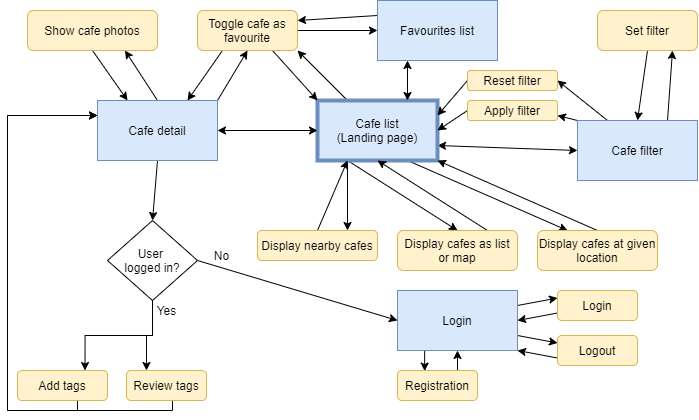
\includegraphics[width=0.9\textwidth]{img/analysis/task-list-graph.png}
    \caption{Coffee Time Task Graph}
    \label{fig:task-graph}
\end{figure}

Because the task list can become very long, it is usually transformed into a \textit{task graph}. The task graph does not have any specific definition, but it should contain every task along with each available screen within the application. Coffee Time's task graph is listed in \Cref{fig:task-graph}. The blue rectangles are screens and the yellow ones are any task what users can do. The application's~entry point is highlighted with bold blue rectangle.

A note about \textit{User Interface Design (MI-NUR)} subject which was held during the winter semester of the academic year of 2019/2020. The Coffee Time prototype was crate as a semester work. Sincere gratitude to classmates \textit{Bc. Ondřej John} and \textit{Bc. Vojtěch Polcar} for their co-working on the prototype. Furthermore, much appreciation to \textit{Ing. Jiří Hunka} for feedback and guidance during the work. The classmates helped during prototyping, proposing functionalities, researching and testing. The High-Fidelity prototype was implemented only by the thesis author. 

\subsubsection{Low Fidelity Prototype}
As a task graph was defined, the Lo-Fi prototype could be made. Although the application is considered as multi-platform application, the prototype was focused on Android, and its Material design \cite{material-design}. The inspiration was taken from typical Material layouts, such as AppBar with title and subsequent actions or tabs the bottom of the screen. 

First of all, the rough prototype was drawn on paper. Its purpose was to come up with some ideas and considered layout. After that, the \textit{Balsamiq} \cite{balsamiq} prototyping software was used. The \textit{Balsamiq} tries to mimic pencil and paper. The prototype is created with a set of components which looks like they are drawn by hand.
The most important feature was the ability to create deep links between screens or components. With a few clicks, the prototype was able to handle actions such as the open application menu or navigate to detail. With that tool, the clickable prototype focused on essential app's features was created. As a result, the PDF was exported. The PDF is enclosed as part of the thesis located at \verb|prototype/lofi.pdf|. The portion of the result is shown in~\Cref{fig:lofi}.

\begin{figure}[htp]
    \centering
    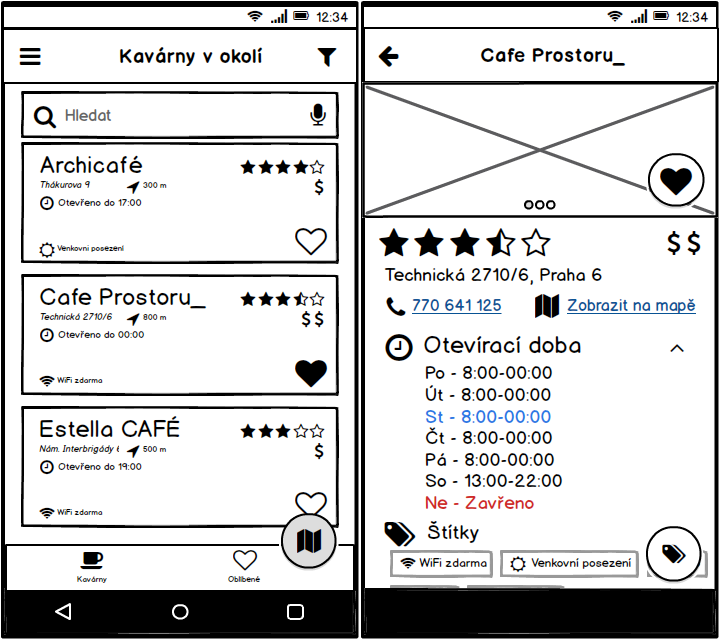
\includegraphics[width=0.75\textwidth]{img/analysis/lofi.png}
    \caption{\gls{lofi} prototype. Cafe list (left) and detail screen (right).}
    \label{fig:lofi}
\end{figure}

The result was tested with co-workers and closest author's family members. From the testing session, useful feedback was given, which is listed along with short answers. 

\begin{questions}
  \item On the cafe list, what if the cafe has more tags than it can display in the row. How to solve it? 
         \begin{answer}
          The solution is to calculate free screen space and display portion of available tags.
         \end{answer}

  \item Research more on how to solve user's reviews.
         \begin{answer}
         As a considered data source is Google Places API, it was acknowledged that it is not possible to add custom reviews through their API.
         \end{answer}
    \item Navigation and contact buttons are too small. 
        \begin{answer}
        Taken into account during implementation.
        \end{answer}
    \item If the tag in detail is clicked, the cafe list with the given tag is shown.
        \begin{answer}
        Taken into account as a valuable tip.
        \end{answer}
    \item Focus on usability with mobile devices, mainly when the user's walk or are in public transport.
        \begin{answer}
        The usability should be more tested. 
        \end{answer}
    \item Focus more to provide understandable information about what tag is and how to use it.
     \begin{answer}
        Information and usability should be more revisited.
    \end{answer}
\end{questions}

\subsubsection{High Fidelity Prototype}
The \gls{hifi} prototype was created as Flutter application. Because of that, in the future, the already written code could be reused. The aim was to create a fully functional prototype for Android devices. As was said earlier in this chapter, the aim of \gls{hifi} is to provide an application so it behaves as real one, which is mainly focused on user interface interaction. That means that the~application does not have any real communication with back-end services. For Coffee Time there was prepared local JSON data source with randomly generated cafe names and their data. Besides that, a few, real one cafes were added to be less general and more known for potential testers. The \gls{hifi} focused on all earlier described use cases. The cafe list screen and cafe's detail screen is shown~in~\Cref{fig:hifi}. The prototype's source code can be found at~\verb|https://github.com/petrnymsa/coffee-time/releases/tag/prototype|~\cite{hifi-prototype}. 

\begin{figure}[htp]
    \centering
    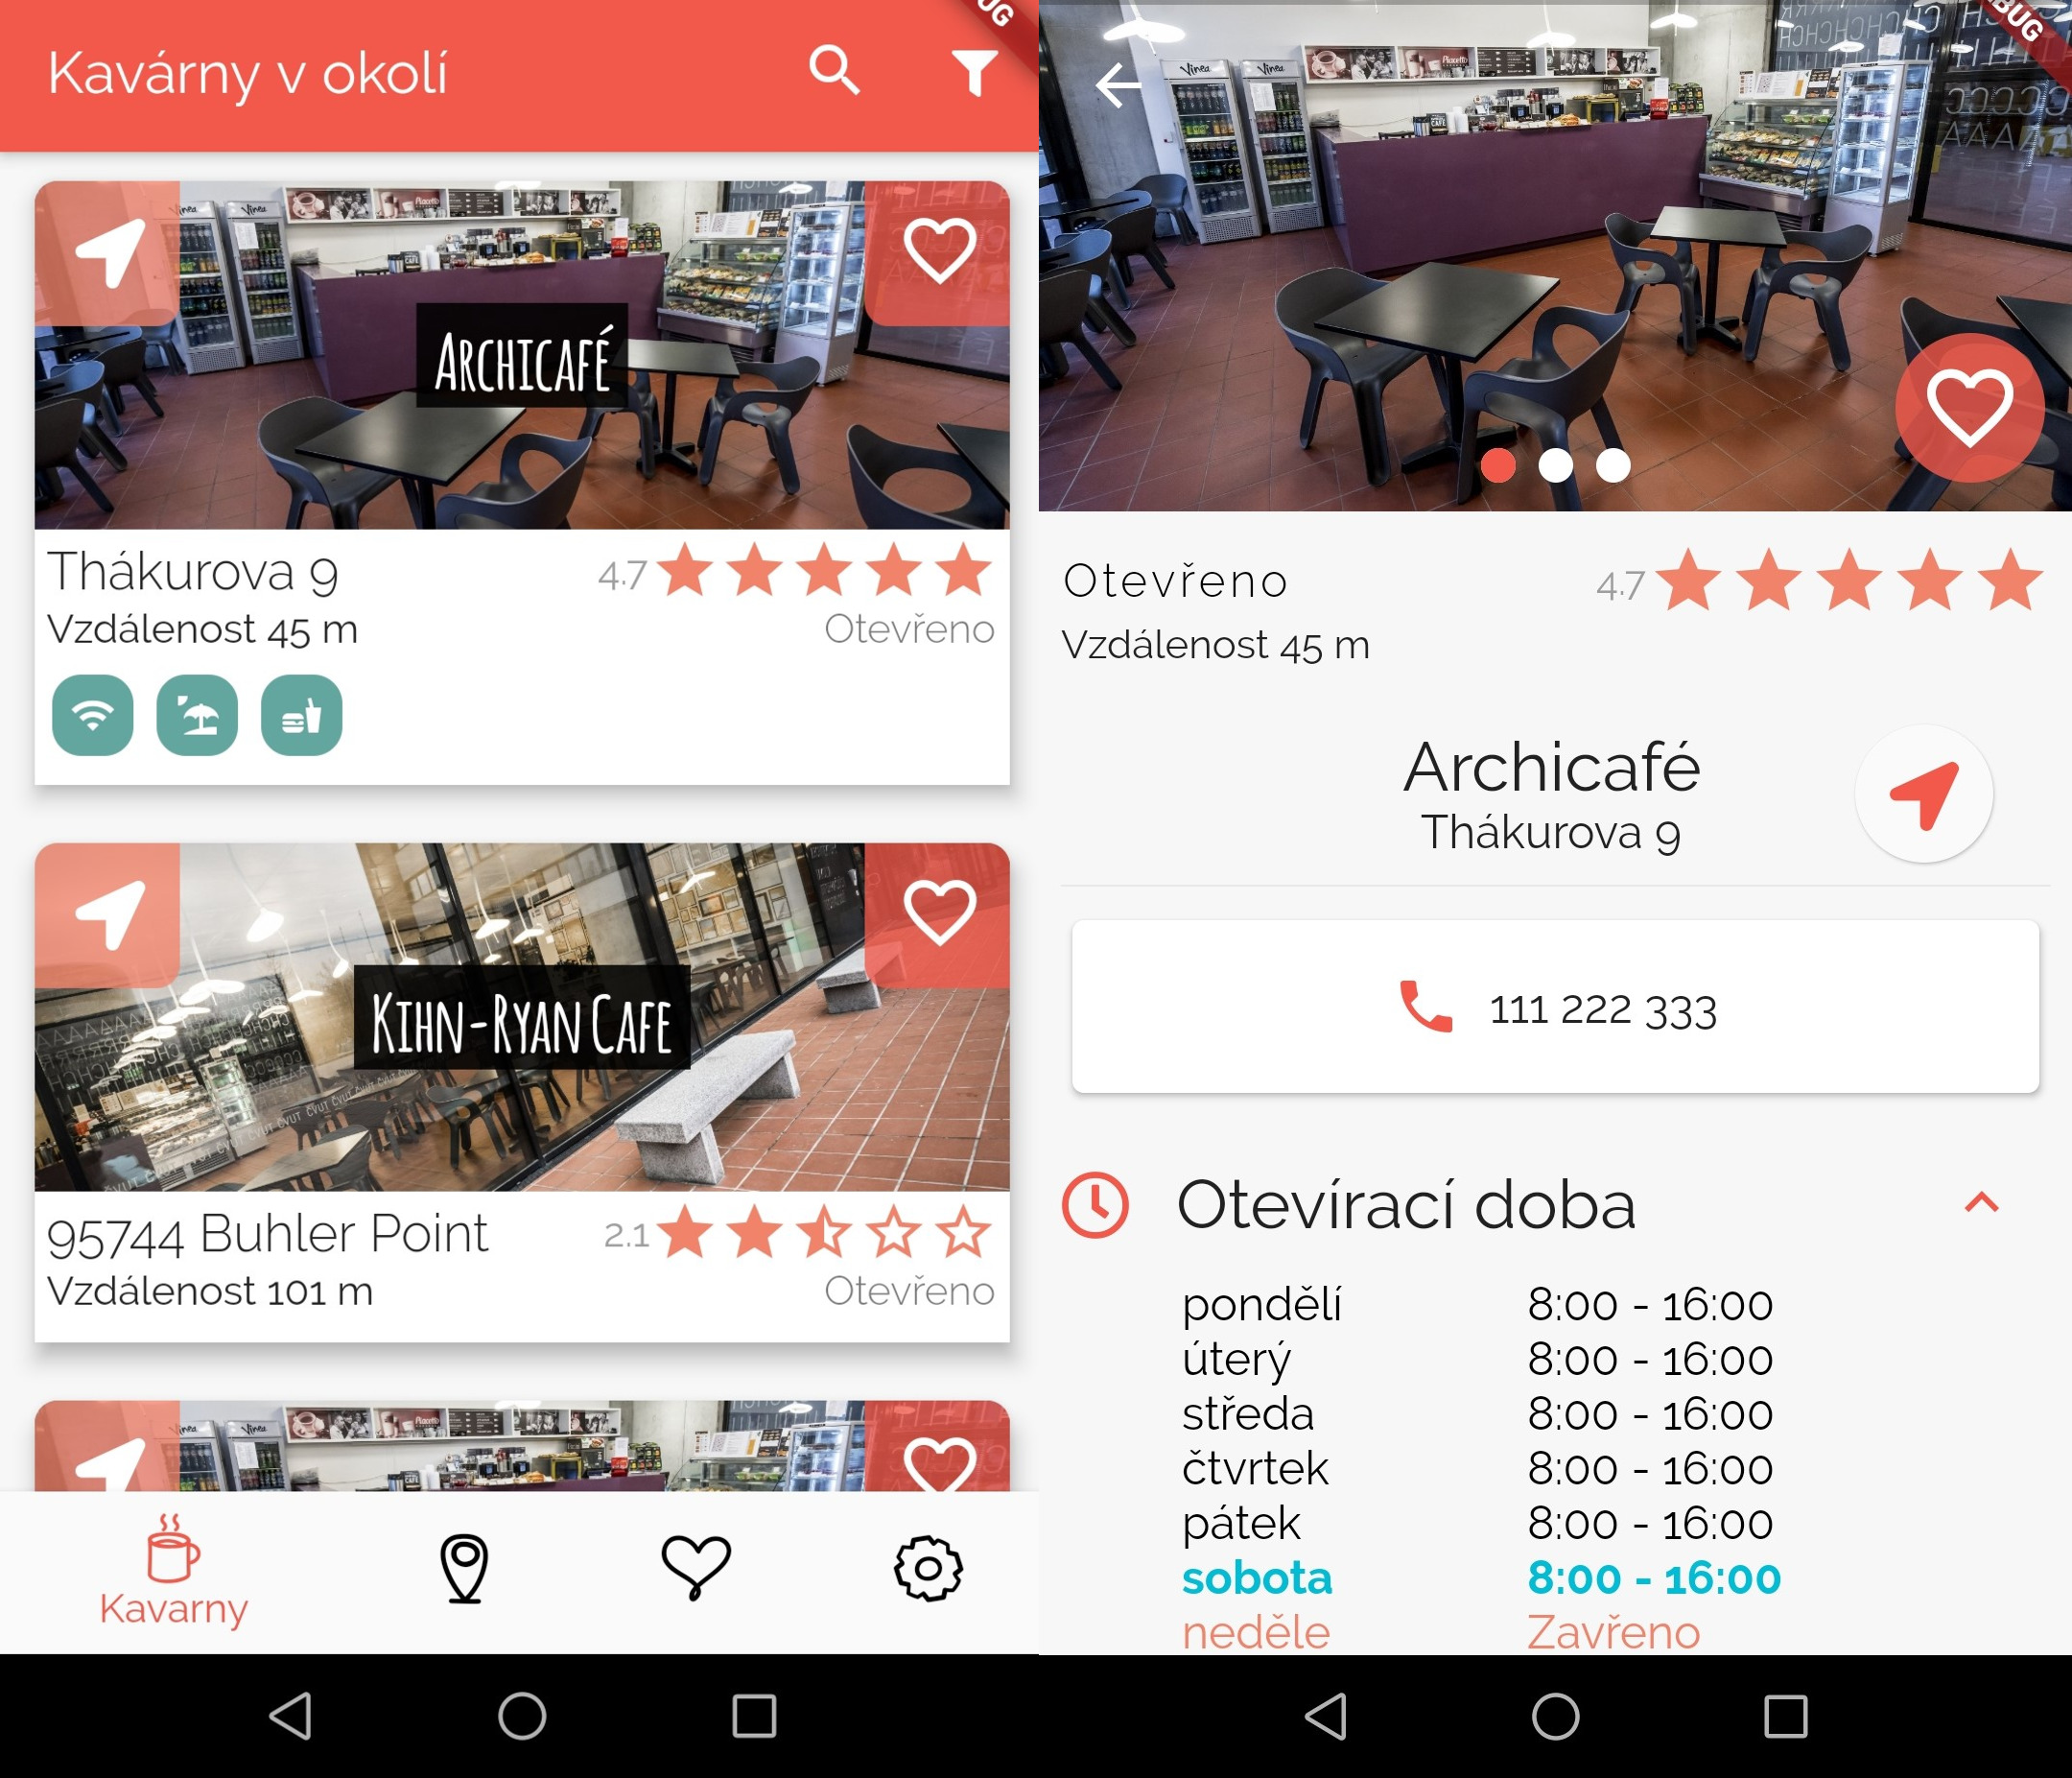
\includegraphics[width=0.6\textwidth]{img/analysis/hifi.jpg}
    \caption{\gls{hifi} prototype. Cafe list (left) and detail screen (right).}
    \label{fig:hifi}
\end{figure}
% --- # --- # --- # --- # --- # --- # --- # --- # --- # --- # --- # --- # --- # --- # --- # --- # --- # --- #
\subsection{Nielsen Heuristic}
\textit{Nielsen Heuristic}~\cite{nielsen} is a usability engineering method for finding the usability problems in a user interface design so that they can be attended to as a part of an iterative design process. The heuristic evaluation involves a small set of rules and these rules should be judged by a small group of ``evaluators''.

Following lines describe one of each of ten rules. Each description is taken from article~\cite{nielsen}.

\begin{enumerate}
    \item \textbf{Visibility of system status} -- The system should always keep users informed about what is going on through appropriate feedback within a reasonable time. 
    
    \item \textbf{Match between system and the real world} -- The system should speak the users' language, with words, phrases and concepts familiar to the user, rather than system-oriented terms. Follow real-world conventions, making information appear in a natural and logical order.
    
    \item \textbf{User control and freedom} -- Users often choose system functions by mistake and will need a clearly marked "emergency exit" to leave the unwanted state without having to go through an extended dialogue. Support undo and redo.
    
    \item \textbf{Consistency and standards} -- Users should not have to wonder whether different words, situations, or actions mean the same thing.
    
    \item \textbf{Error prevention} -- Even better than good error messages is a careful design which prevents a problem from occurring in the first place. Either eliminate error-prone conditions or check for them and present users with a confirmation option before they commit to the action.
    
    \item \textbf{Recognition rather than recall} -- Minimize the user's memory load by making objects, actions, and options visible. The user should not have to remember information from one part of the dialogue to another. Instructions for the use of the system should be visible or easily retrievable whenever appropriate.
    
    \item \textbf{Flexibility and efficiency of use} -- Accelerators — unseen by the novice user — may often speed up the interaction for the expert user such that the system can cater to both inexperienced and experienced users. Allow users to tailor frequent actions.
    
    \item \textbf{Aesthetic and minimalist design} -- Dialogues should not contain information which is irrelevant or rarely needed. Every extra unit of information in a dialogue competes with the relevant units of information and diminishes their relative visibility.
    
    \item \textbf{Help users recognise, diagnose, and recover from errors} -- Error messages should be expressed in plain language (no codes), precisely indicate the problem, and constructively suggest a solution.
    
    \item \textbf{Help and documentation} -- Even though it is better if the system can be used without documentation, it may be necessary to provide help and documentation. Any such information should be easy to search, focused on the user's task, list concrete steps to be carried out, and not be too large.
\end{enumerate}
% --- & --- & --- & --- & --- & --- & --- & --- & --- & --- & --- & --- & --- & --- & --- & --- & --- & --- &
\subsubsection{Coffee Time Evaluation}
During \textit{MI-NUR} lecture, the above-described heuristic was evaluated against \gls{hifi} prototype. Each screen was taken individually and judged with all rules. Note that only found rules violation are described for each screen.

\begin{itemize}
    \item Cafe list
    \begin{itemize}
        \item Rule \#2: Some tags icons are hard to understand, and their meaning can be easily misunderstood. 
        \item Rule \#8: When filtering is on, it occupies nearly one-third of the screen.
        \item Rule \#9: There is no visible error handling for missing internet connection or location services.
    \end{itemize}
    \item Favourites cafes
    \begin{itemize}
        \item Rule \#2: Same as Cafe list.
        \item Rule \#3: When a favourite cafe is set off, there is no indication that action is permanent without the ability to undoing it. 
    \end{itemize}
    \item Detail screen
    \begin{itemize}
        \item Rule \#2: Same as Cafe list.
        \item Rule \#6: It is not clear how to start navigation. This functionality is provided by the button to the right of the cafe's address. There should be a more visible indication that this action is possible.
    \end{itemize}
    \item Map  screen -- No rules violation found. 
    \item Filter screen -- The only violation is the same as within Cafe list about icons.
\end{itemize}

Once the violations are found, they should be prioritised. The priority indicates how serious violation is. The more severe violation, the more unusable is it for users. The priorities are: 

\begin{itemize}
    \item 1 -- negligible,
    \item 2 -- visible issue,
    \item 3 -- the usability can suffer,
    \item 4 -- frustrating experience,
    \item 5 -- User is not able to use application at all.
\end{itemize}

The most violated rule is number \#2 with tag icons. With this issue suffer most of the screen, because icons are used very often.  This issue has priority 3.  The second issue with favourites cafes (priority 2) can be solved, for example, with small notification with the undo button. The prototype does not have implemented any kind of error handling regarding internet connection or location services (priority 2). 
% --- # --- # --- # --- # --- # --- # --- # --- # --- # --- # --- # --- # --- # --- # --- # --- # --- # --- #
\subsection{User Testing}
The prototype was tested with seven testers. An important note is that four testers are people who have ``IT knowledge'' and are classmates from university. It was assumed that their understanding could vary against other testers.

The process of testing was as follows -- application was launched on a real device. Each testing was recorded. The recording was essential to know what testers thought, how they used the application and behaved. Each user had the same set of use case scenarios, and the supervisor did not interact either provide any advice to testers how to proceed. There was only one exception when the supervisor was allowed to advise, and that was when tester did not know how to proceed -- he became ``totally lost''. This situation could indicate two different things. First, from the test case scenario, it was not particularly evident what tester should do. Secondly, the test case was understandable, but the application interface not. The second problem is more important for the testing and the results.  The test case scenario can be rewritten or with the help of supervisor fully explained. 

The description of test case scenarios, along with established issues, follows. Each test case has an introduction for users in which situation they are.  Next contains test case goal, expected user behaviour and actual behaviour. Note that, the actual behaviour is not part of this summarization. Instead of, the~found issues are summarised. 
% --- & --- & --- & --- & --- & --- & --- & --- & --- & --- & --- & --- & --- & --- & --- & --- & --- & --- &
\subsubsection{Test Case 1: Favourite Cafe}
An user visits his favourite cafe and he would like to add this Cafe to his favourite list. 
\begin{itemize}
    \item \textbf{Goal} -- Add Cafe to favourites.
    \item \textbf{Expected behaviour}
    \begin{enumerate}
        \item An user is located on the cafe list screen. The targeted cafe is displayed.
        \item An user clicks on the heart icon located in top right corner of the cafe's tile. 
        \item Alternative flow: An user is located on detail screen and taps heart icon located on the top of the screen. 
    \end{enumerate}
    \item \textbf{Found Issues} -- The testers went through a test case without any issues.
\end{itemize}
% --- & --- & --- & --- & --- & --- & --- & --- & --- & --- & --- & --- & --- & --- & --- & --- & --- & --- &
\subsubsection{Test Case 2: Start Navigation to Selected Cafe}
An user has selected cafe and wants to navigation to the cafe's location.
\begin{itemize}
    \item \textbf{Goal} -- Start navigation.
    \item \textbf{Expected behaviour}
    \begin{enumerate}
        \item An user is located on the cafe list screen. The targeted cafe is displayed.
        \item An user clicks on the navigation icon located in top left corner of the cafe's tile. 
        \item Alternative flow: An user is located on the detail screen and taps navigation icon located to the right of address.
    \end{enumerate}
    \item \textbf{Found Issues}
    \begin{enumerate}
        \item Three different icons used to start navigation. Icon is different on the cafe list from icon within detail screen.
        \item In the detail screen, it is not clear that icon can start navigation.
    \end{enumerate}
    \item \textbf{Proposed solution}
    \begin{enumerate}
        \item Use same icon everywhere.
        \item The same problem stated in the Nielsen heuristic evaluation. The icon should be highlighted. Can be added ``elevation''~\cite{material-design-elevation} -- shadow under the component to provide depth. 
    \end{enumerate}
\end{itemize}
% --- & --- & --- & --- & --- & --- & --- & --- & --- & --- & --- & --- & --- & --- & --- & --- & --- & --- &
\subsubsection{Test Case 3: Filter Cafes with Tags}
An user is interested in cafes where they offer beside the coffee has also beer.
\begin{itemize}
    \item \textbf{Goal} -- Filter Cafes that has ``beer'' tag.
    \item \textbf{Expected behaviour}
    \begin{enumerate}
        \item On the cafe list screen, an user selects filter icon to open filter screen.
        \item Within filter screen, an user selects to filter by tags and choose ``beer''.
        \item User confirms the filter. 
    \end{enumerate}
    \item \textbf{Found Issues}
    \begin{enumerate}
        \item ``Filter screen is confusing. Confirmation is useless.''
        \item ``Do not open filter screen, just open some modal window to selects tags''.
        \item The filter icon is unclear.
        \item ``If the user is located on the detail screen, clicking on the tag icon should set the~ filter.'' 
    \end{enumerate}
    \item \textbf{Proposed solution}
    \begin{enumerate}
        \item The filter icon is standardised icon. 
        \item Clicking on tag should set the filter. 
    \end{enumerate}
\end{itemize}
% --- & --- & --- & --- & --- & --- & --- & --- & --- & --- & --- & --- & --- & --- & --- & --- & --- & --- &
\subsubsection{Test Case 4: Suggest New Tag}
An user visits regularly cafe which is friendly to dog owners. The user found out that this information is missing in the application. 
\begin{itemize}
    \item \textbf{Goal} -- The user suggests tag ``dog friendly'' or similar for the cafe. 
    \item \textbf{Expected behaviour}
    \begin{enumerate}
        \item An user selects cafe and opens detail screen.
        \item An user clicks on ``suggest change''.
        \item An user adds tag ``dog friendly'' and confirms suggestion.
    \end{enumerate}
    \item \textbf{Found Issues} -- No issues found.
\end{itemize}
% --- & --- & --- & --- & --- & --- & --- & --- & --- & --- & --- & --- & --- & --- & --- & --- & --- & --- &
\subsubsection{Test Case 5: Tag review}
An user visits regularly cafe which has mistaken information about ``available parking''. He would like to inform about this wrong tag. 
\begin{itemize}
    \item \textbf{Goal} -- The user should review ``parking'' with dislike. 
    \item \textbf{Expected behaviour}
    \begin{enumerate}
        \item An user selects cafe and opens detail screen.
        \item An user clicks on ``suggest change''.
        \item An user reviews ``parking'' with dislikes and confirms suggestion. 
    \end{enumerate}
    \item \textbf{Found Issues} -- No issues found.
\end{itemize}
% --- & --- & --- & --- & --- & --- & --- & --- & --- & --- & --- & --- & --- & --- & --- & --- & --- & --- &
\subsubsection{Test Case 6: Most popular nearby cafe}
An user wants find the most popular cafe around him. 
\begin{itemize}
    \item \textbf{Goal} -- The user change ordering from ``by distance'' to ``by popularity''.
    \item \textbf{Expected behaviour}
    \begin{enumerate}
        \item An user opens filter screen.
        \item An user changes to ordering by popularity.
        \item An user confirms filter.
    \end{enumerate}
    \item \textbf{Found Issues} -- No issues found.
\end{itemize}

From testers was obtained beneficial feedback which helps to tune user interface for better usability. Besides feedback from individual test cases, a few additional tips were given.

\begin{itemize}
    \item Cafe's name on tile can be harder to read with the contrasting background image. \textit{Can be solved with making photo darker.}
    \item Landscape mode is not working. \textit{During prototype it wasn't considered.}
    \item The map marker could contain more information than cafe's name.
\end{itemize}

All feedback was gathered and was taken into account during the next phase of implementation.
% ----- % ----- % ----- % ----- % ----- % ----- % ----- % ----- % ----- % ----- % ----- % ----- % ----- % ----- %
\section{Back-end Analysis}
In this section, the technical analysis of available technologies for back-end services is discussed. The focus is only on the back-end part. The technical detail of the mobile application is discussed in the next~\Cref{ch:implementation}.

One vital part of the whole architecture is~\gls{gpa}~\cite{google-places-api}. This API offers access to Google Maps services, searching places, place details, place photos and more. The API has five services~\cite{google-places-api}. 

\begin{itemize}
    \item Place search -- a list of places based on the user's location or search query.
    \item Place details -- returns more detail information about a specific place.
    \item Place photos -- provides access to place-related photos.
    \item Place autocomplete -- automatically fills in the name or address of a place.
    \item Query autocomplete -- provides a query prediction service for text-based geographic searches.
\end{itemize}

To access these services, the Google~API~Key must be obtained~\cite{google-places-api-key}.
% --- # --- # --- # --- # --- # --- # --- # --- # --- # --- # --- # --- # --- # --- # --- # --- # --- # --- #
\subsection{Google Places API}
The Google Places API returns plenty of information about each place, but the application uses an only subset of available information. The application makes usage of four available services -- Find a place, Nearby search, Place detail and Place photos. Some parameters are the same for each service, and the output of each service is similar. 
Each place has several fields such as name, address, location, rating and much more. However, not every field is used in the application, and it is not necessary to obtain these fields in the response. On top of that, each field is included in the pricing category. That means that some of the fields are more expensive to obtain than others~\cite{google-places-api-billing}. It was important to analyse which fields are essential to get before the API model could be created. Following lines summarise each API usage, its parameters, fields and expected output.
% --- & --- & --- & --- & --- & --- & --- & --- & --- & --- & --- & --- & --- & --- & --- & --- & --- & --- &
\subsubsection{Find Place}
The purpose of this service is to find places based on the text-based query or custom location. \Cref{table:gapi-find-place-params} describes each used parameter. \Cref{table:gapi-find-place-fields} describes each expected field in the response. 

\begin{table}[htbp]
\centering
\begin{tabularx}{\textwidth}{|l|X|}
\hline
\textbf{Parameter} & \textbf{Usage}                                                    \\ \hline
key                & API key                                                           \\ \hline
input              & search query                                                      \\ \hline
inputtype          & set to textquery                                                  \\ \hline
language           & language code                    \\ \hline
locationbias       & set to circle:radius@lat,lng.                                     \\ \hline
\end{tabularx}
\caption{Find place parameters}
\label{table:gapi-find-place-params}
\end{table}
% ------
\begin{table}[htbp]
\centering
\begin{tabularx}{\textwidth}{|l|X|}
\hline
\textbf{Field}     & \textbf{Description}                                                      \\ \hline
place\_id          & unique place identification                                                \\ \hline
name               & place's name                                                              \\ \hline
icon               & place's icon                                                              \\ \hline
geometry           & geolocated latitude,longitude                                             \\ \hline
formatted\_address & human-readable address                                                    \\ \hline
types              & list of place categories such as ``cafe''                                 \\ \hline
photos             & contains photo width, height and photo\_reference                          \\ \hline
opening\_hours     & contains only open\_now. For full information, detail request is required \\ \hline
price\_level       & value from 0 to 4                                                         \\ \hline
rating             & value from 1.0 to 5.0                                                     \\ \hline
\end{tabularx}
\caption{Find place fields}
\label{table:gapi-find-place-fields}
\end{table}
% --- & --- & --- & --- & --- & --- & --- & --- & --- & --- & --- & --- & --- & --- & --- & --- & --- & --- &
\subsubsection{Nearby Search}
\textit{Nearby Search} allows finding nearby places around the given location. In contrast with \textit{Find place}, the \textit{Nearby Search} returns all fields available to place and can return up to~60~places. The result is paginated~up~to three pages with~20~places in each page. If the result has another page, the pagetoken is included in the response. As before~\Cref{table:gapi-nearby-search-parameters} shows service parameters.

\begin{table}[htbp]
\centering
\begin{tabularx}{\textwidth}{|l|X|}
\hline
\textbf{Parameter} & \textbf{Usage} \\ \hline
key                & API key \\ \hline
location           & latitude,longtitude \\ \hline
radius             & circular radius in meters, max 50 000m  \\ \hline
language           & language code \\ \hline
opennow         & place should be open. If place does not have this field, it is omitted from results  \\ \hline
type & place type, always set to \textit{cafe} \\ \hline
pagetoken & token for next page \\ \hline 
\end{tabularx}
\caption{Nearby Search parameters}
\label{table:gapi-nearby-search-parameters}
\end{table}
% --- & --- & --- & --- & --- & --- & --- & --- & --- & --- & --- & --- & --- & --- & --- & --- & --- & --- &
\subsubsection{Place Details}
Each place has additional information accessible through place details. \Cref{table:gapi-details-parameters} describes each parameter used, and~\Cref{table:gapi-find-place-fields} describes fields which should be returned in the response.

\begin{table}[htbp]
\centering
\begin{tabularx}{\textwidth}{|l|X|}
\hline
\textbf{Parameter} & \textbf{Usage} \\ \hline
key                & API key \\ \hline
place\_id           & place's id \\ \hline
language           & language code \\ \hline
\end{tabularx}
\caption{Place Details parameters}
\label{table:gapi-details-parameters}
\end{table}

\begin{table}[htbp]
\centering
\begin{tabularx}{\textwidth}{|l|X|}
\hline
\textbf{Parameter} & \textbf{Usage} \\ \hline
international\_phone\_number           & phone number in international format \\ \hline
opening\_hours           & opening times and if is currently open \\ \hline
photos                & additional up to ten photos \\ \hline
review           & up to five user reviews \\ \hline
utc\_offset           &  offset in minutes from UTC \\ \hline
website           & place's website \\ \hline
\end{tabularx}
\caption{Place Details fields}
\label{table:gapi-details-fields}
\end{table}

Note that \textit{opening\_hours} contains localised \textit{weekday\_text}. If a place is always open, the \textit{close} field within \textit{opening\_hours} is missing and \textit{open} field has day equal to zero and time equal to ``0000''.
% --- & --- & --- & --- & --- & --- & --- & --- & --- & --- & --- & --- & --- & --- & --- & --- & --- & --- &
\subsubsection{The API Response Format}
The \gls{gpa} can respond with \textit{JSON} or \textit{XML} format. The \textit{JSON} format was chosen as a~more typically used and standard format for REST~API and mobile communication~\cite{xml-vs-json}. 

\begin{listing}[h!]
\begin{minted}{json}
{
  "html_attributions": [],
   "results": [      
      {
         "business_status": "OPERATIONAL",
         "id": "0c19db184d6705e945686f3d83ae02a3fbf23068",
         "name": "JS Café",
         "opening_hours": {
            "open_now": true
         },
      }
   ],
   "status": "OK"
}
\end{minted}
\caption{Nearby Search example output (shortened).}
\label{listing:gapi-example-response}
\end{listing}

The \textit{Find Place}, \textit{Nearby Search} and \textit{Place Details} has similar response format where \verb|<status>| indicates response code because \gls{gpa} for each request always responds with HTTP status code 200~OK. The status field can have several values such as \verb|OK| for successful request, \verb|ZERO_RESULTS| for empty results or \verb|INVALID_REQUEST| for general invalid request. Each service has different result field name -- \verb|candidates| for \textit{Find Place}, \verb|results| for \textit{Nearby Search} and~\verb|result| for \textit{Place Details}. An~example output is shown~in~\Cref{listing:gapi-example-response}.
% --- & --- & --- & --- & --- & --- & --- & --- & --- & --- & --- & --- & --- & --- & --- & --- & --- & --- &
\subsubsection{Place Photos}
Each place can have photos. The response from \textit{Find Place} or \textit{Nearby Search} contains \verb|photo_reference| along with width and height of the photo. For~obtaining actual photo itself, the~\textit{Place Photos} endpoint must be called. The~endpoint accepts as always the \verb|key| (API key) and \verb|photo_reference|. The~result can be altered with parameters for maximal width or height. Returns byte-encoded image if the request was successful otherwise HTTP status code ``\textit{400 Bad Request}'' or ``\textit{403 Forbidden}'' if the quota limit was reached. 

Although Google Places API returns plenty of information about each place, one added benefit of the Coffee Time application is user suggested tags. This requirement cannot be fulfilled only with Places API, so there is a requirement for another, custom, API. 
% --- # --- # --- # --- # --- # --- # --- # --- # --- # --- # --- # --- # --- # --- # --- # --- # --- # --- #
\subsection{Coffee Time API}
The~\gls{cta} will be used for two main functionalities. First of all, it will provide access to Google Places API and secondly, it will be used for getting assigned tags for cafes. While it is possible to use \gls{gpa} directly from the mobile application (client), it would lead to the~need for another request to obtain the~cafe's tags and another possible required custom information. Hence, if custom API is used as a~proxy to~\gls{gpa}, with one request to this API, the response can be modified with additional data and returned at~once. \Cref{fig:api-communication} shows such a~communication. 

\begin{figure}[ht]
    \centering
    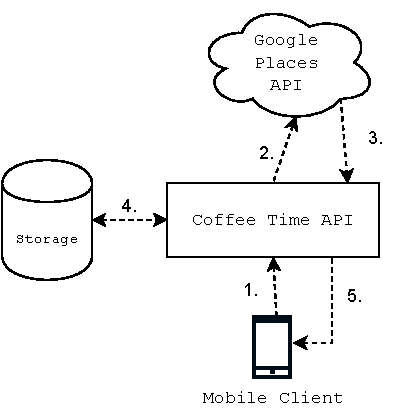
\includegraphics[width=0.5\linewidth]{img/analysis/api-communication-flow.pdf}
    \caption{Client and API communication flow}
    \label{fig:api-communication}
\end{figure}

\begin{enumerate}
    \item HTTP request made by client to Coffee Time API.
    \item The request is processed and redirected to Google Places API.
    \item The response from Google Places API is obtained.
    \item If appropriate the query to storage is issued, and response is enhanced with obtained data.
    \item The final result is returned to the client.
\end{enumerate}
% --- & --- & --- & --- & --- & --- & --- & --- & --- & --- & --- & --- & --- & --- & --- & --- & --- & --- &
\subsubsection{The Cafe Tags}

\begin{figure}[ht]
    \centering
    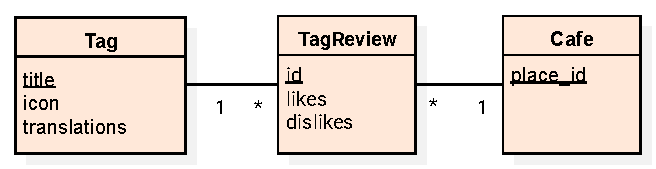
\includegraphics[width=0.8\linewidth]{img/analysis/tag-cafe-relation.pdf}
    \caption{Cafe's tag and Cafe relation}
    \label{fig:tag-cafe-relation}
\end{figure}

The set of available tags is predefined, with the requirement to be able to change it any time without changes within the client or in~the API. Each tag has a~title and an icon and can be translated into another language. This definition and requirement for no changes within the client imply that used icon has to be part of tag's definition in the~\gls{cta}. To sum up, each tag is an entity with a unique title, icon and translation. 

As was said earlier in this chapter, each cafe can have assigned tags. Each assigned tag is reviewed by users with the concept of ``likes'' and ``dislikes''.  This requirement implies that for each cafe is needed to be known assigned tags and their reviews. This relation is shown in~\Cref{fig:tag-cafe-relation}.
% --- & --- & --- & --- & --- & --- & --- & --- & --- & --- & --- & --- & --- & --- & --- & --- & --- & --- &
\subsubsection{Domain Model}
Within detail screen, additional information is displayed, which can be obtained from the Place Details call. This concludes that the application's cafe domain entity is split into two entities - Cafe and Cafe Detail entities. The~domain entity graph is listed in~\Cref{fig:domain} showing all entities related to~\gls{cta} response.

\begin{figure}[ht]
    \centering
    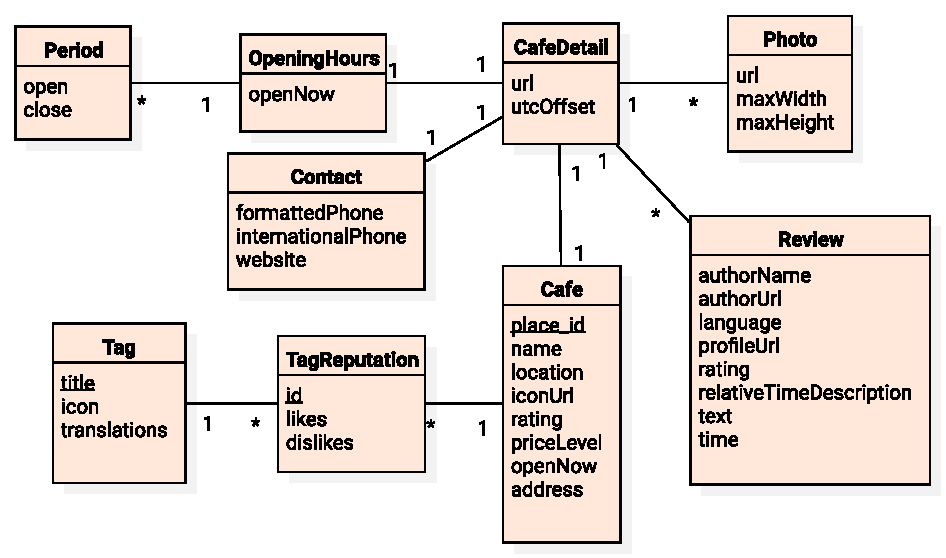
\includegraphics[width=0.9\linewidth]{img/analysis/domain.pdf}
    \caption{Coffee Time domain model}
    \label{fig:domain}
\end{figure}
% --- & --- & --- & --- & --- & --- & --- & --- & --- & --- & --- & --- & --- & --- & --- & --- & --- & --- &

% --- # --- # --- # --- # --- # --- # --- # --- # --- # --- # --- # --- # --- # --- # --- # --- # --- # --- #
\subsection{The Selection of the Right Technology}
The technology which will be used to build the API should fulfil the following requirements:

\begin{itemize}
    \item The access to API should be secured,
    \item The back-end service should be simply scaled up when needed,
    \item The maintenance cost should be kept low.
\end{itemize}

There are many technologies which can be used to achieve this requirements. One of the ways is implementing API from the ground with technologies such as \textit{.NET Core} and its \textit{ASP .NET Core API}. Then the~API can be deployed to service hosting providers such as~\textit{Microsoft Azure} or through technologies such as Docker containers and Kubernetes~\cite{kubernetes} as container orchestration. 

Another way is to use serverless services. The serverless is approach where ``the cloud provider is responsible for executing a piece of code by dynamically allocating the resources. And only charging for the amount of resources used to run the code. The code is typically run inside stateless containers that can be triggered by a variety of events including http requests, database events, queuing services, monitoring alerts, file uploads, scheduled events (cron jobs), etc''~\cite{what-is-serverless}. This approach is sometimes called as \textit{Functions as a Service} (FaaS in short). The major providers are \textit{Amazon Web Services} and its \textit{Lambda Functions}, \textit{Microsoft Azure Functions} or \textit{Cloud Functions (Firebase Functions)} by \textit{Google}. 

The~\textit{Firebase} by~\textit{Google} is collection of services which helps to build mobile application faster, improve application quality and grow business. The~\textit{Firebase} offer services as real-time NoSQL database, application usage analytics, A/B user testing, cloud web hosting or Cloud Functions and much more. Within one service, the storage for data, the API as functions and security can be made. 
% --- & --- & --- & --- & --- & --- & --- & --- & --- & --- & --- & --- & --- & --- & --- & --- & --- & --- &
\subsubsection{Cloud Firestore}
\textit{Cloud Firestore} is a flexible, scalable database for mobile, web, and server development. It keeps data in sync across client apps through realtime listeners and offers offline support for mobile and web. The \textit{Cloud Firestore} uses NoSQL data model. The data are stored in documents that contain fields mapping to values. These documents are stored in collections, which are containers for documents that are used to organize data. Documents support many different data types, from simple strings and numbers, to complex, nested objects. Documents can include subcollections and build hierarchical data structures that scale as database grows~\cite{cloud-firestore}.
% --- & --- & --- & --- & --- & --- & --- & --- & --- & --- & --- & --- & --- & --- & --- & --- & --- & --- &
\subsubsection{Cloud Functions}
\textit{Cloud Functions} for \textit{Firebase} is a serverless framework that lets automatically run backend code in response to events triggered by Firebase and HTTPS requests. After function is deployed, Google's servers begin to manage the function immediately. The~function can be used directly with an HTTP request. Each function runs in isolation, in its own environment with its own configuration and are scaled accordingly to usage load~\cite{cloud-functions}. 
% --- & --- & --- & --- & --- & --- & --- & --- & --- & --- & --- & --- & --- & --- & --- & --- & --- & --- &
\subsubsection{Firebase Authentication}
\textit{Firebase Auth} offers service to secure application with \textit{OAuth~2.0} standard~\cite{oauth}. It automatically integrates with identity providers such as \textit{Google}, \textit{Microsoft}, \textit{Facebook} and more. Besides that it offers standard authentication through user's email or phone~\cite{cloud-auth} and anonymous authentication where for each user randomly generated identifier is used. The~service guarantees that for each user, as long they use the same device, the identifier stays the same. 
\\
\\
The~\textit{Cloud Functions} can be used to build Coffee Time API. The~\textit{Cloud Firestore} as a database (storage) and API can be secured through \textit{Firebase Authentication}. On top of that, \textit{Firebase} offers services for analysis, logging and user testing. The~\textit{Firebase} has ``pay as you go'' model and offers a free plan (Spark plan). The Spark plan offers up to 1~GiB data storage, 20~thousands of writes and 50~thousand of document reads per day. The~\textit{Cloud Functions} can be invoked 125~thousand times per month. This pricing perfectly suits the requirements and can be used freely to build Coffee Time application. If the application becomes popular and frequently used, the actual price of \textit{Firebase} services is calculated by current usage and services can be scaled up accordingly. How the \textit{Firebase} services are used in detail is more described in~\Cref{ch:implementation}. 

% ----- % ----- % ----- % ----- % ----- % ----- % ----- % ----- % ----- % ----- % ----- % ----- % ----- % ----- %
\section{The Conclusion}
In this chapter, the considered application Coffee Time was introduced. The analysis of existing alternatives was made to obtain inspiration for how each application behaves. The prototype was created to propose user interface and tested it with users. In the end, the analysis of Coffee Time API was made along with analysis of chosen technology to build this API.

\chapter{Implementation}
\label{ch:implementation}
\todo{introduction}
\blind[1]

\section{High level app overview}
\todo{api, mobile client, express.js, admin SDK, place api}

\section{Coffee Time API}
\todo{express.js, api communication, ...}

\section{Coffee Time}
\todo{intro}

\todo{the art of clean architecture}

\todo{domain layer}

\todo{data layer}

\todo{repository layer}

\subsection{Representation Layer}
\todo{representation layer}

\todo{screens}
\todo{bloc, states, events, ... sealed union, freezed}


\chapter{User testing}
\todo{Beta user testing. Experiments and results}

\todo{What todo? No real testing done as planned... thank you COVID-19, only a few friends tested app,...}

\todo{Dev process? Github, open issue, Continuous Integration? Open-source?}

\begin{conclusion}
In the first chapter, the Flutter framework as a new promising cross-platform framework was introduced. How the framework works, its philosophy ``everything is a widget'' was explained and different approaches of state management were discussed. 

Next chapter was focused on introducing proposed application, on its designing process, prototyping and user testing. As was described, Low-Fidelity and High-Fidelity prototypes were created to verify proposed design. Both prototypes are also included along with final implementation in the appendix. 

In the implementation, more details were covered and also introduced several popular packages and solutions within Flutter community. In the end, \textit{Android} version was successfully tested and released for everyone. 

\section{Next Steps}
Coffee Time is for sure not ``feature-complete'' and there is plenty of space to improvements. Ongoing future development is planned to obtain more experience with Flutter framework and bring an even better, feature ``rich'', application. 

Next possible features and steps can be:

\begin{itemize}
    \item Add missing feature ``searching cafes in custom location''.
    \item Synchonization of favorited cafes.
    \item Better map view with more information in it.
    \item Optimise application performance, responsivity and adaptability to different form factors, screen sizes and resolutions.
    \item Add full \textit{iOS} support. This includes redesign of the application to more modern cross-platform look. 
    \item As a experiment, build application also for web and desktop platform.
\end{itemize}

Personal author's note to the end

\begin{quote}
I really believe that Flutter is a promising framework, which increasingly gains on popularity and in the closest future there will be more opportunities as the framework will get adopted by larger companies. In contrast with Xamarin, my subjective opinion is that the Flutter development workflow is faster, more convenient and easier to use. Of course, as with every new popular framework, there is no guarantee that Flutter will be truly the right solution in the future. I believe that at this moment companies can use Flutter for applications, which do not require specific platform functionalities, such as virtual reality, without any doubt.
\end{quote}
\end{conclusion}

\bibliographystyle{iso690.bst}
\bibliography{ref.bib}

\appendix

%\chapter{Seznam použitých zkratek}
\printglossaries

\chapter{Content of enclosed CD \todo{USB?}}

Vhodným způsobem vizualizujte obsah přiloženého média. Lze použít balíček \verb|dirtree| a vytvořit např. následující výstup (adresáře src a text s~příslušným obsahem jsou \emph{povinné}):

\begin{figure}
	\dirtree{%
		.1 readme.txt\DTcomment{stručný popis obsahu CD}.
		.1 exe\DTcomment{adresář se spustitelnou formou implementace}.
		.1 src.
		.2 impl\DTcomment{zdrojové kódy implementace}.
		.2 thesis\DTcomment{zdrojová forma práce ve formátu \LaTeX{}}.
		.1 text\DTcomment{text práce}.
		.2 thesis.pdf\DTcomment{text práce ve formátu PDF}.
	}
\end{figure}


\end{document}
